\documentclass[final]{beamer}
%% \title{Energy and Growth, History and Dynamics}
%\title{Economic development with unlimited supplies of energy:
%\\The English Industrial Revolution and modern economic growth}

\title{Third ECE Conference\\Aberystwyth, Wales\\July 2013} %for 2103 ECE Aberyswyth
\author{Stephen C. Bannister\\
	Department of Economics\\
	University of Utah\\
	Salt Lake City, Utah 84112\\
	USA\\
	\href{mailto:steve.bannister@econ.utah.edu}{steve.bannister@econ.utah.edu}\\
	}

%\date{Drafts May 2012,}
\date{}
\usepackage[latin1]{inputenc}
%\usepackage[english]{babel}
\usepackage{amsmath}
\usepackage{amsfonts}
\usepackage{txfonts}
\usepackage{amssymb}
\usepackage{pgfpages}
\usepackage{booktabs}
\usepackage{longtable}

\usetheme{Darmstadt}
\usecolortheme{beaver}

\usepackage{chngpage}
%\usepackage{pdfpages}
\usepackage{graphicx}
%\usepackage[lofdepth,lotdepth,position=bottom]{subfig}
\usepackage{caption}
%\usepackage{draftwatermark}

\usepackage{verbatim}
%\usepackage{underscore}
%\linespread{1.9}	% remove for single, 1.3 for 1.5 and 1.6 for 2.0. use this setting for print editing

\usepackage{glossaries}

\graphicspath{{../diss2/images/}}

%\textwidth{7.5in}
%\addtolength{\textwidth}{1.0in} 
%\addtolength{\oddsidemargin}{-0.5in} 
%\addtolength{\evensidemargin}{-0.5in} 
%\addtolength{\textheight}{1.25in}
%\addtolength{\topmargin}{-0.75in}

\setbeamertemplate{navigation symbols}{} %no nav symbols

\usepackage{hyperref}

%\makeglossaries

%\loadglsentries{glossary.tex}

%\setcounter{secnumdepth}{4}%to number paragraphs so can ref them?

\begin{document}

%\SetWatermarkLightness{0.93}
%\SetWatermarkScale{1}

	\maketitle
	\nocite{*}
%	\bibliographystyle{E:/LaTeX-Portable/MikTex-Portable/bibtex/bst/base/IEEEanot}

	\bibliographystyle{E:/LaTeX-Portable/MikTex-Portable/bibtex/bst/base/plain-annote}
%	\bibliographystyle{plain}

\begin{frame}
\begin{itemize}
\item Econonomics -- general, micro/macro unification
\item Welsh economics history
\item Podolinski, Fredrick Soddy
\item Importance of energy
	\begin{itemize}
	\item diss2\_beamer
	\item motion charts
	\end{itemize}
\end{itemize}
\end{frame}

\begin{frame}
\frametitle{What do economists do?}
\begin{itemize}	
\item Attempt to model complex social systems -- Macroeconomics -- lots of equilibrium-based models
\item Attempt to explain individual (consumer/firm) behaviour -- Microeconomics
\item Attempt to link them -- microfoundations of macroeconomics, network systems with emergent behaviours, stochastic agent-based models
\end{itemize}
\end{frame}

\begin{frame}
\frametitle{Similarities/dissimilarities with physics}
\begin{itemize}
\item Use maths in several ways (physics envy?)
	\begin{itemize}
	\item Theory -- so use mostly the same algebras you do (especially linear), although so far no tensor algebra
	\item Applied -- since difficult to repeat experiments, have evolved a wide set of statistical methods
	\item Simulation
	\end{itemize}
\item Use scientific methods, processes (publish, etc.)
\item Share people -- Fredrick Soddy, Wall Streen ``quants''
\item Narrow vein of thermodynamicists (Sergei Podolinski, Georgescu-Roegen) to whom economics is a thermodynamic system
\item Must incorporate institutions and history
\item Again, very little repeatability -- difficult to ``rewind'' a macroeconomy since people are involved
\end{itemize}
\end{frame}

\begin{frame}
\frametitle{English Industrial Revolution, 1590 - 1876}

	\begin{itemize}
	\item Modern economic growth
	\item Unconstrained quantity of fossil carbon energy -- an \textit{energy} revolution led by a demand revolution
	\item Little statistical space for institutional or cultural events -- except to explain structural breaks
	\item Framework applicable across time series, space, and time
	\end{itemize}
\end{frame}

\section{main}

\begin{frame}
\frametitle{Taxonomy of EIR explanations}
\footnotesize{
\begin{table}[p!]
%\caption{Taxonomy of EIR explanations}
\label{tbl:taxonomy}
\begin{tabular}{ll}
Label&Examples\\
\hline \hline
English exceptionalists&Landes (1969), McCloskey (2010), Mokyr (1992,2010)\\
Partial culturalists&Cipolla (1966), Pomeranz (2001), Allen (2009)\\
Primarily energetic&Cottrell (1955), Wrigley (1988,2010), Malanima (2010)\\
Thermodynamicists&Georgescu-Roegen (1975), Ayres (2003), Garrett (2009)\\
\end{tabular}
\end{table}
}
\end{frame}

\begin{frame}
\frametitle{Author/time-span series of energy consumption, GDP, and population}
\begin{figure}[p!]
\center
%\caption{Author/time-span series of energy consumption, GDP, and population}
\label{fig:overall levels}
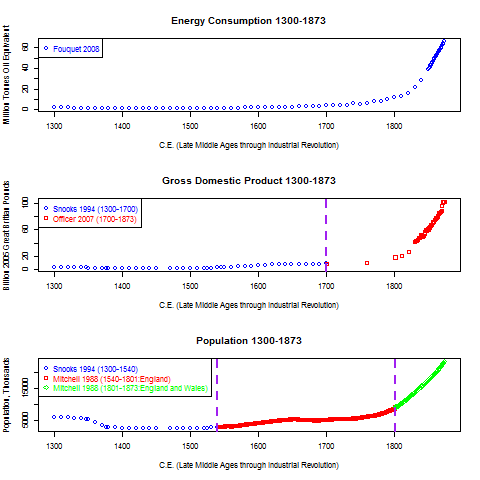
\includegraphics[height=0.8\textheight]{overallLevels}
\end{figure}
\end{frame}

\begin{frame}
\frametitle{English real gross domestic product, \\
levels and per--capita }

		\begin{figure}[p!]
%		\caption{English real gross domestic product, \\
%		levels and per--capita }
		\label{fig:ggdp}		
		\centerline{
		\mbox{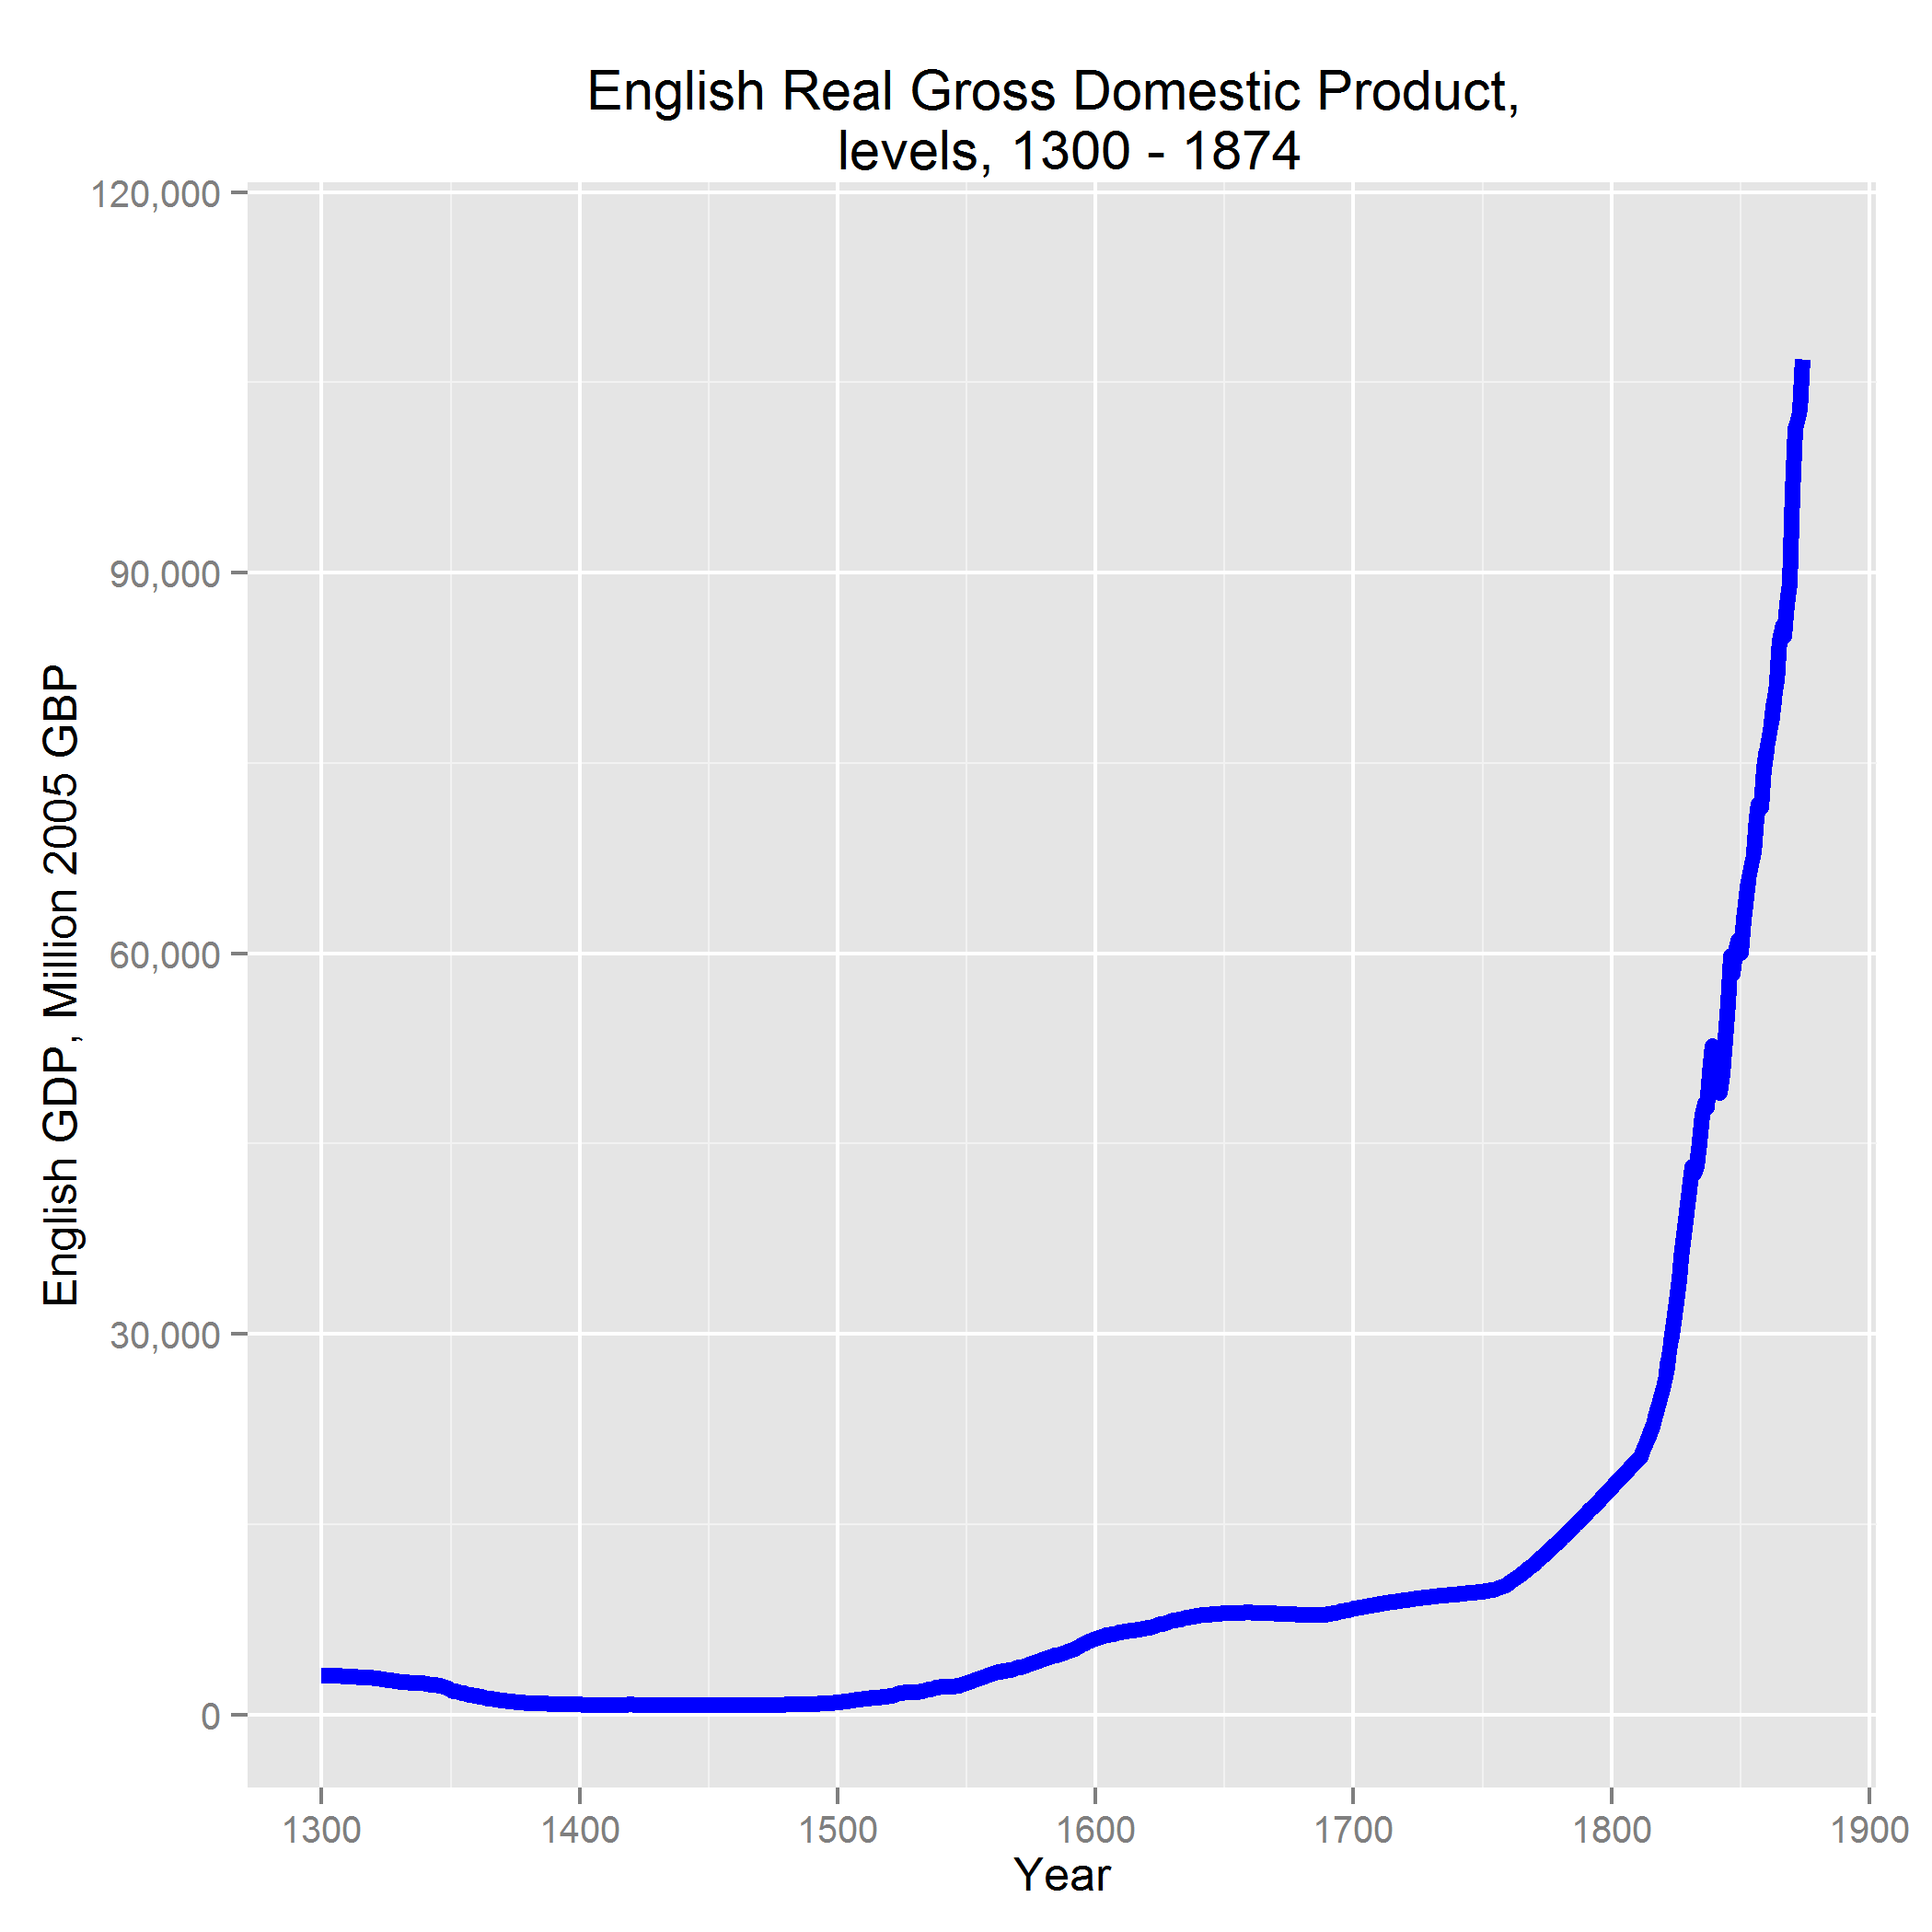
\includegraphics[width=0.55\textwidth]{ggdp}}
		\mbox{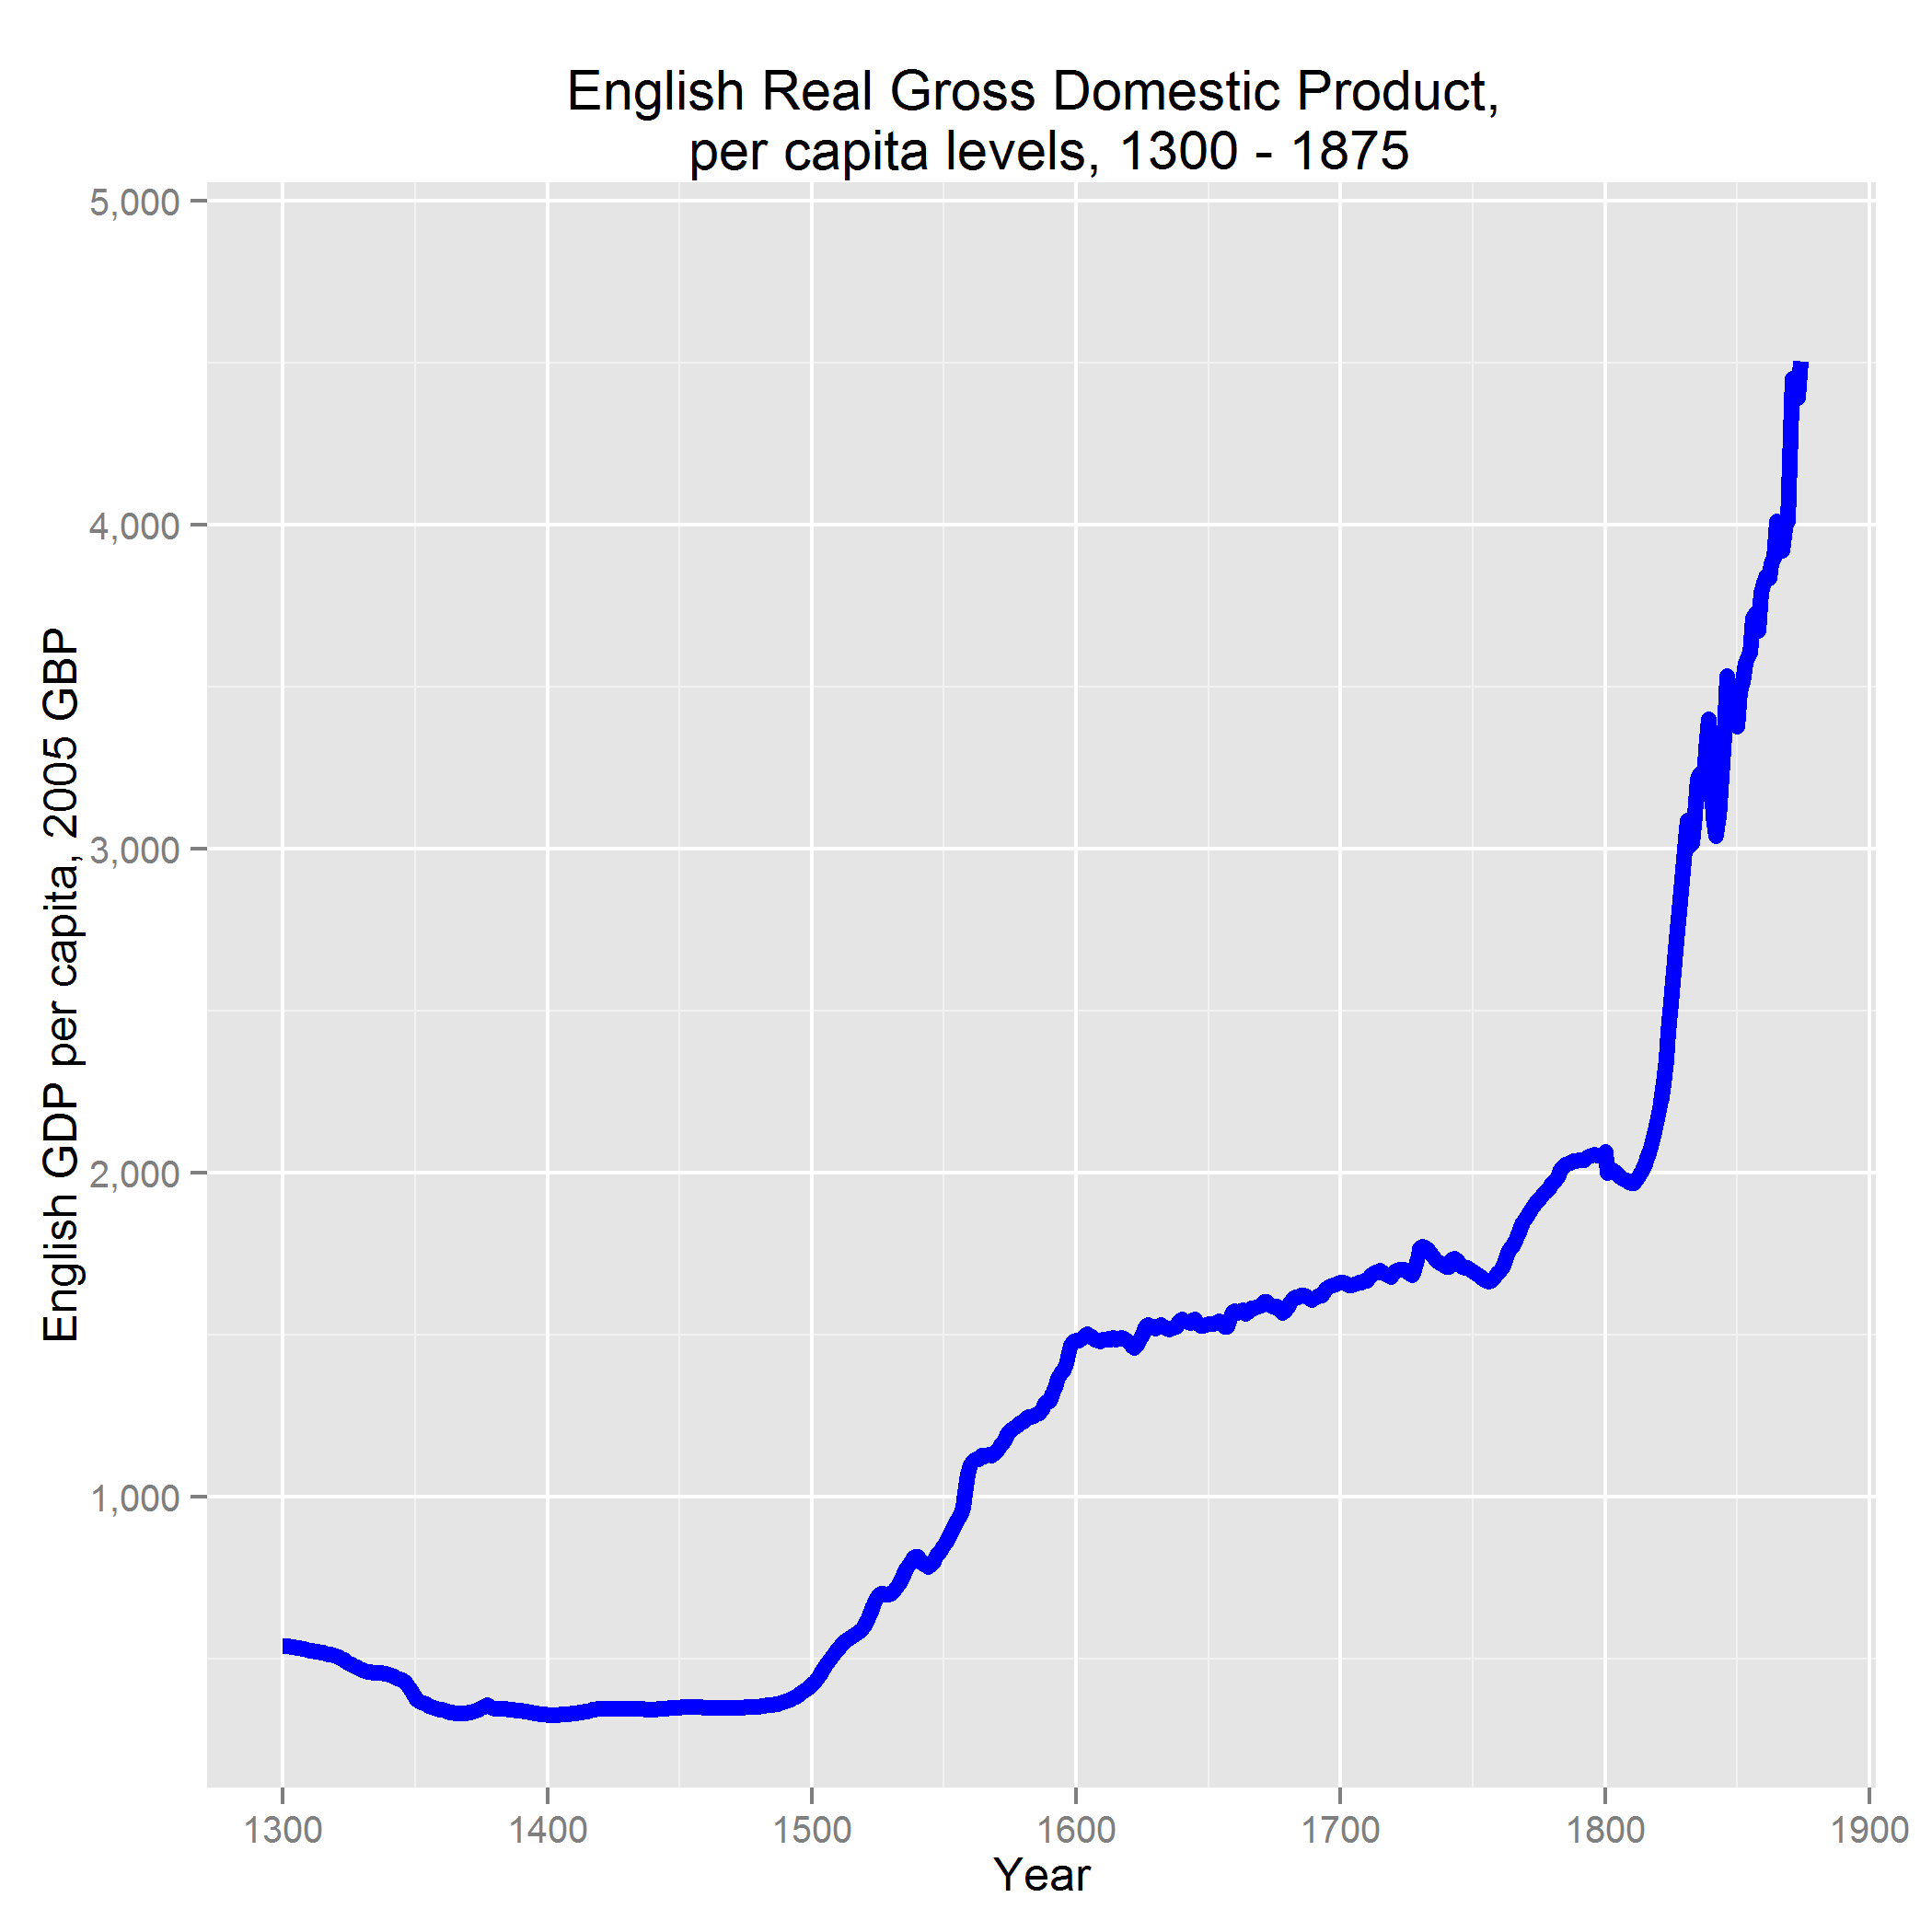
\includegraphics[width=0.55\textwidth]{ggdppop}}
		}
		\end{figure}
\end{frame}

\begin{frame}
		\frametitle{English real gross domestic product, \\
	log levels and log per--capita}

		\begin{figure}[p!]
%		\caption{English real gross domestic product, \\
%		log levels and log per--capita}
		\label{fig:gdpLog}		
		\centerline{
		\mbox{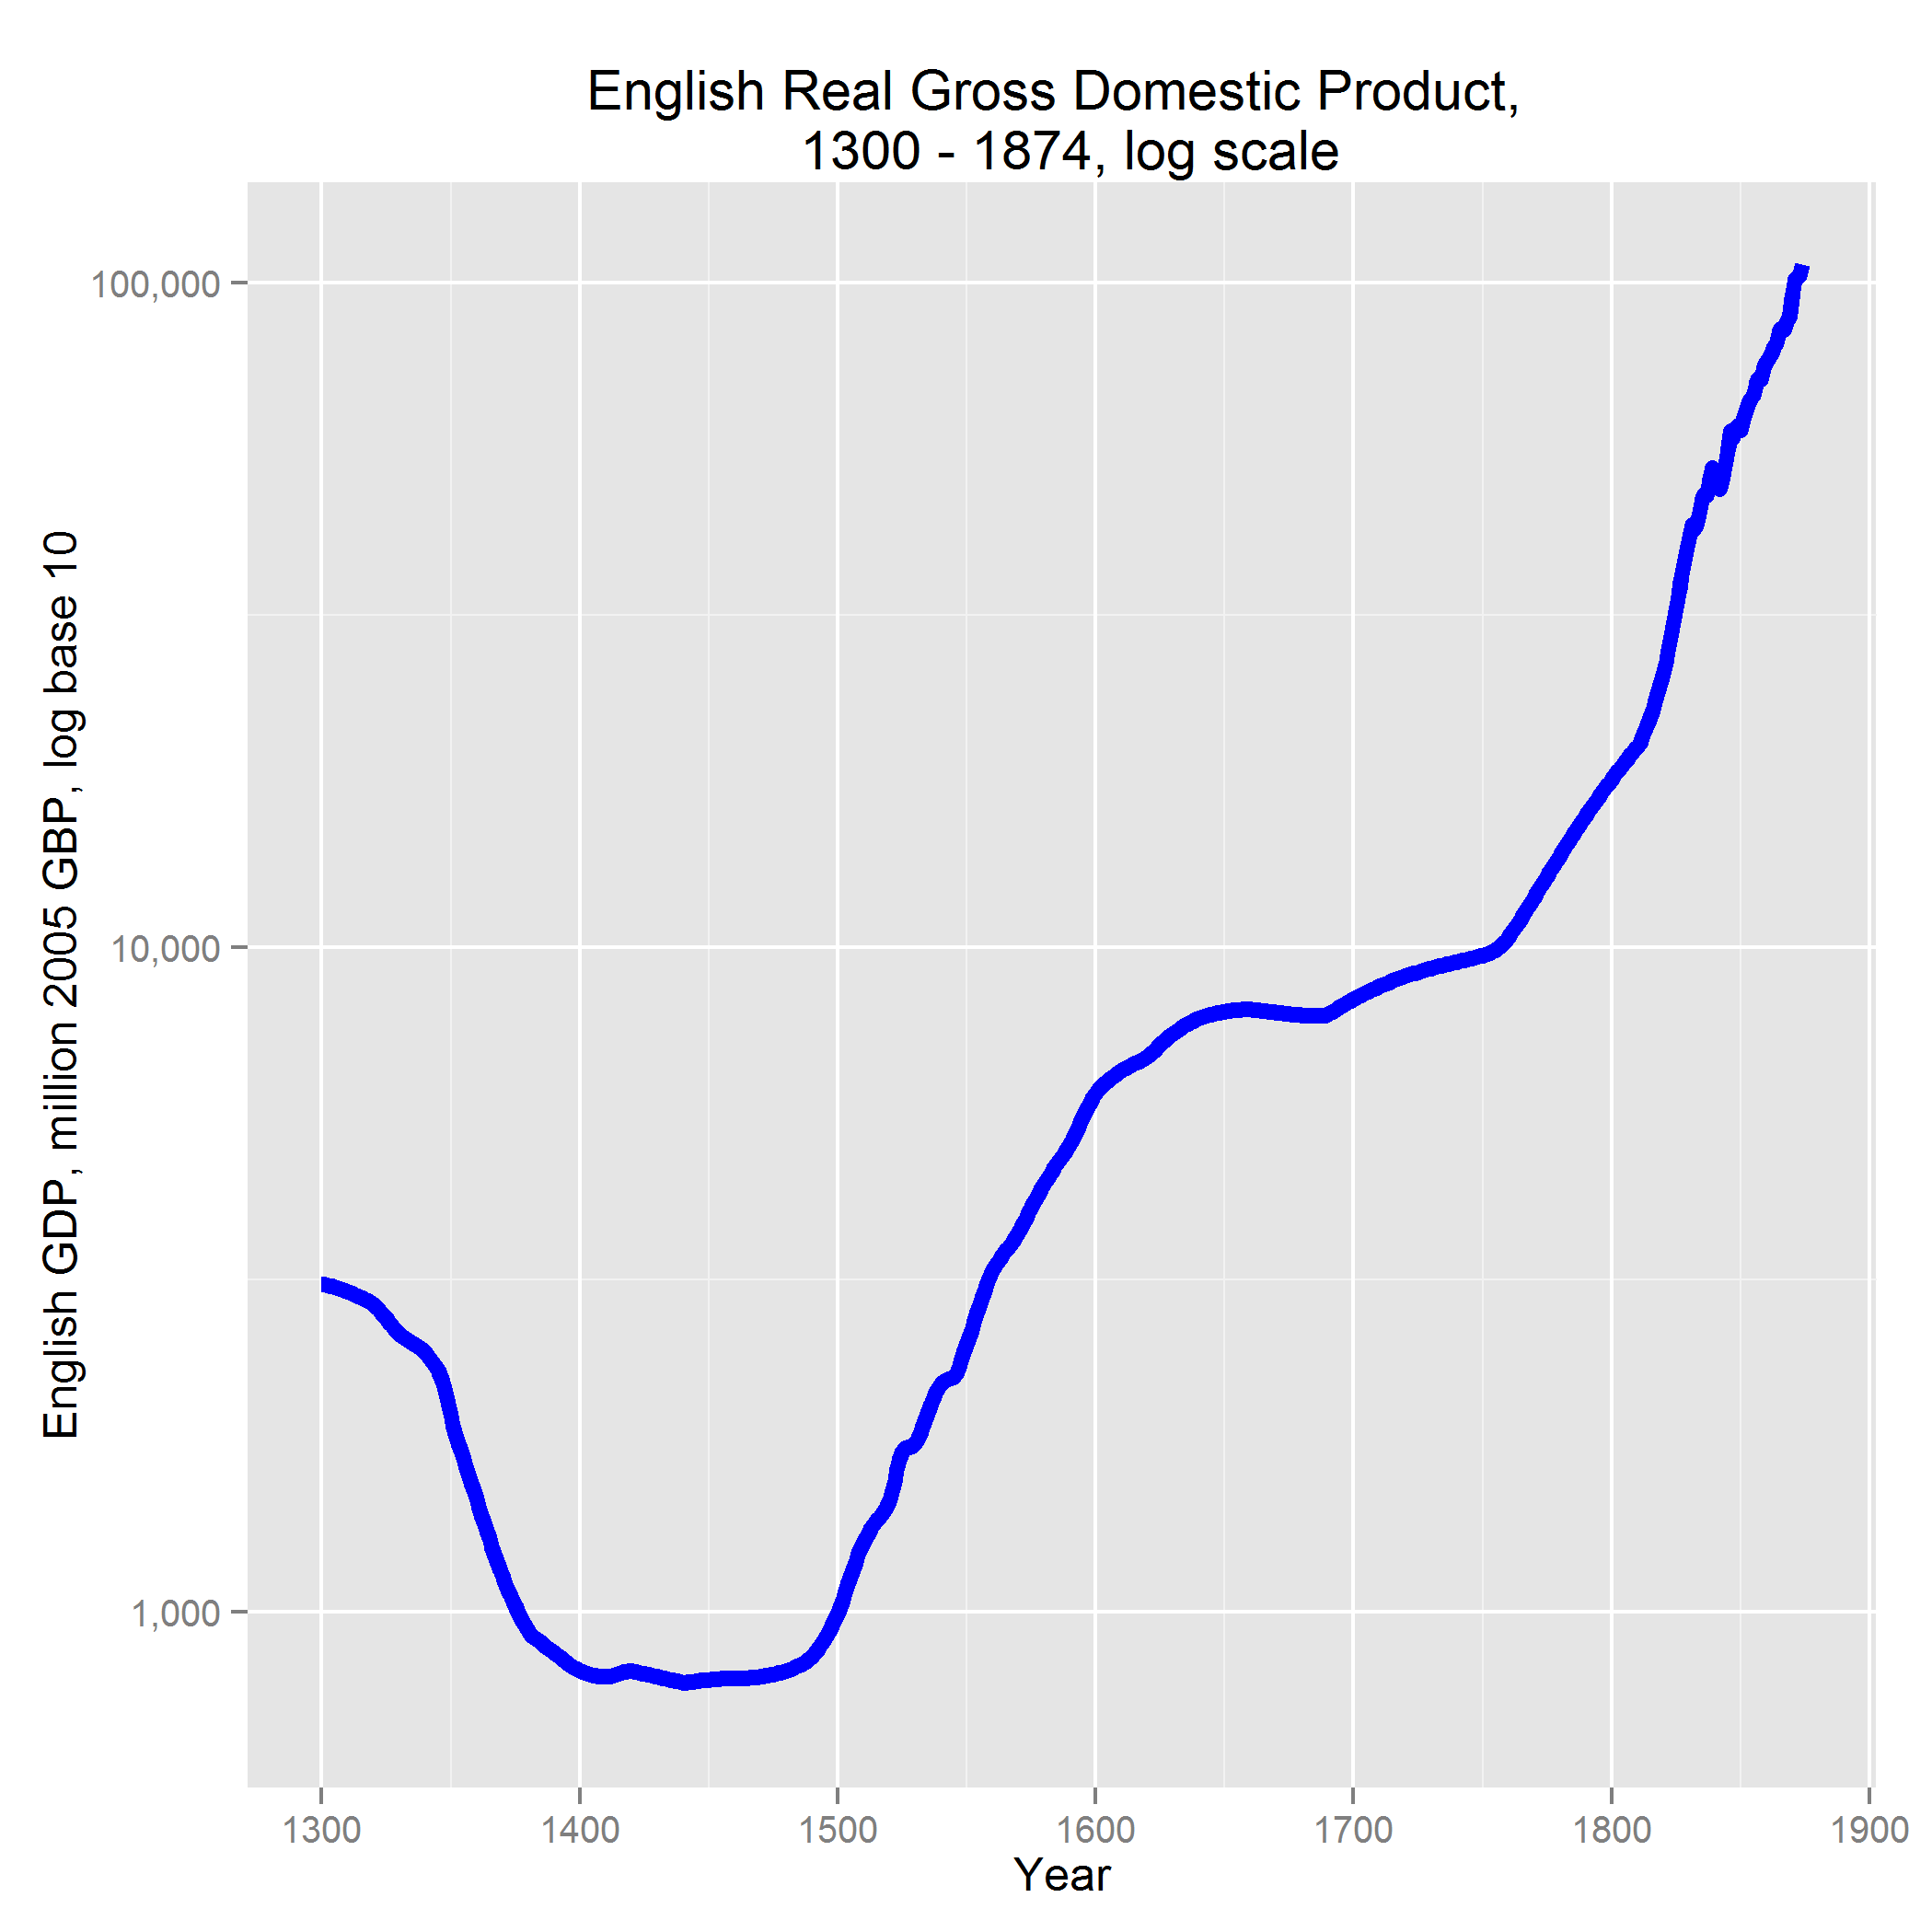
\includegraphics[width=0.55\textwidth]{gdpLog}}
		\mbox{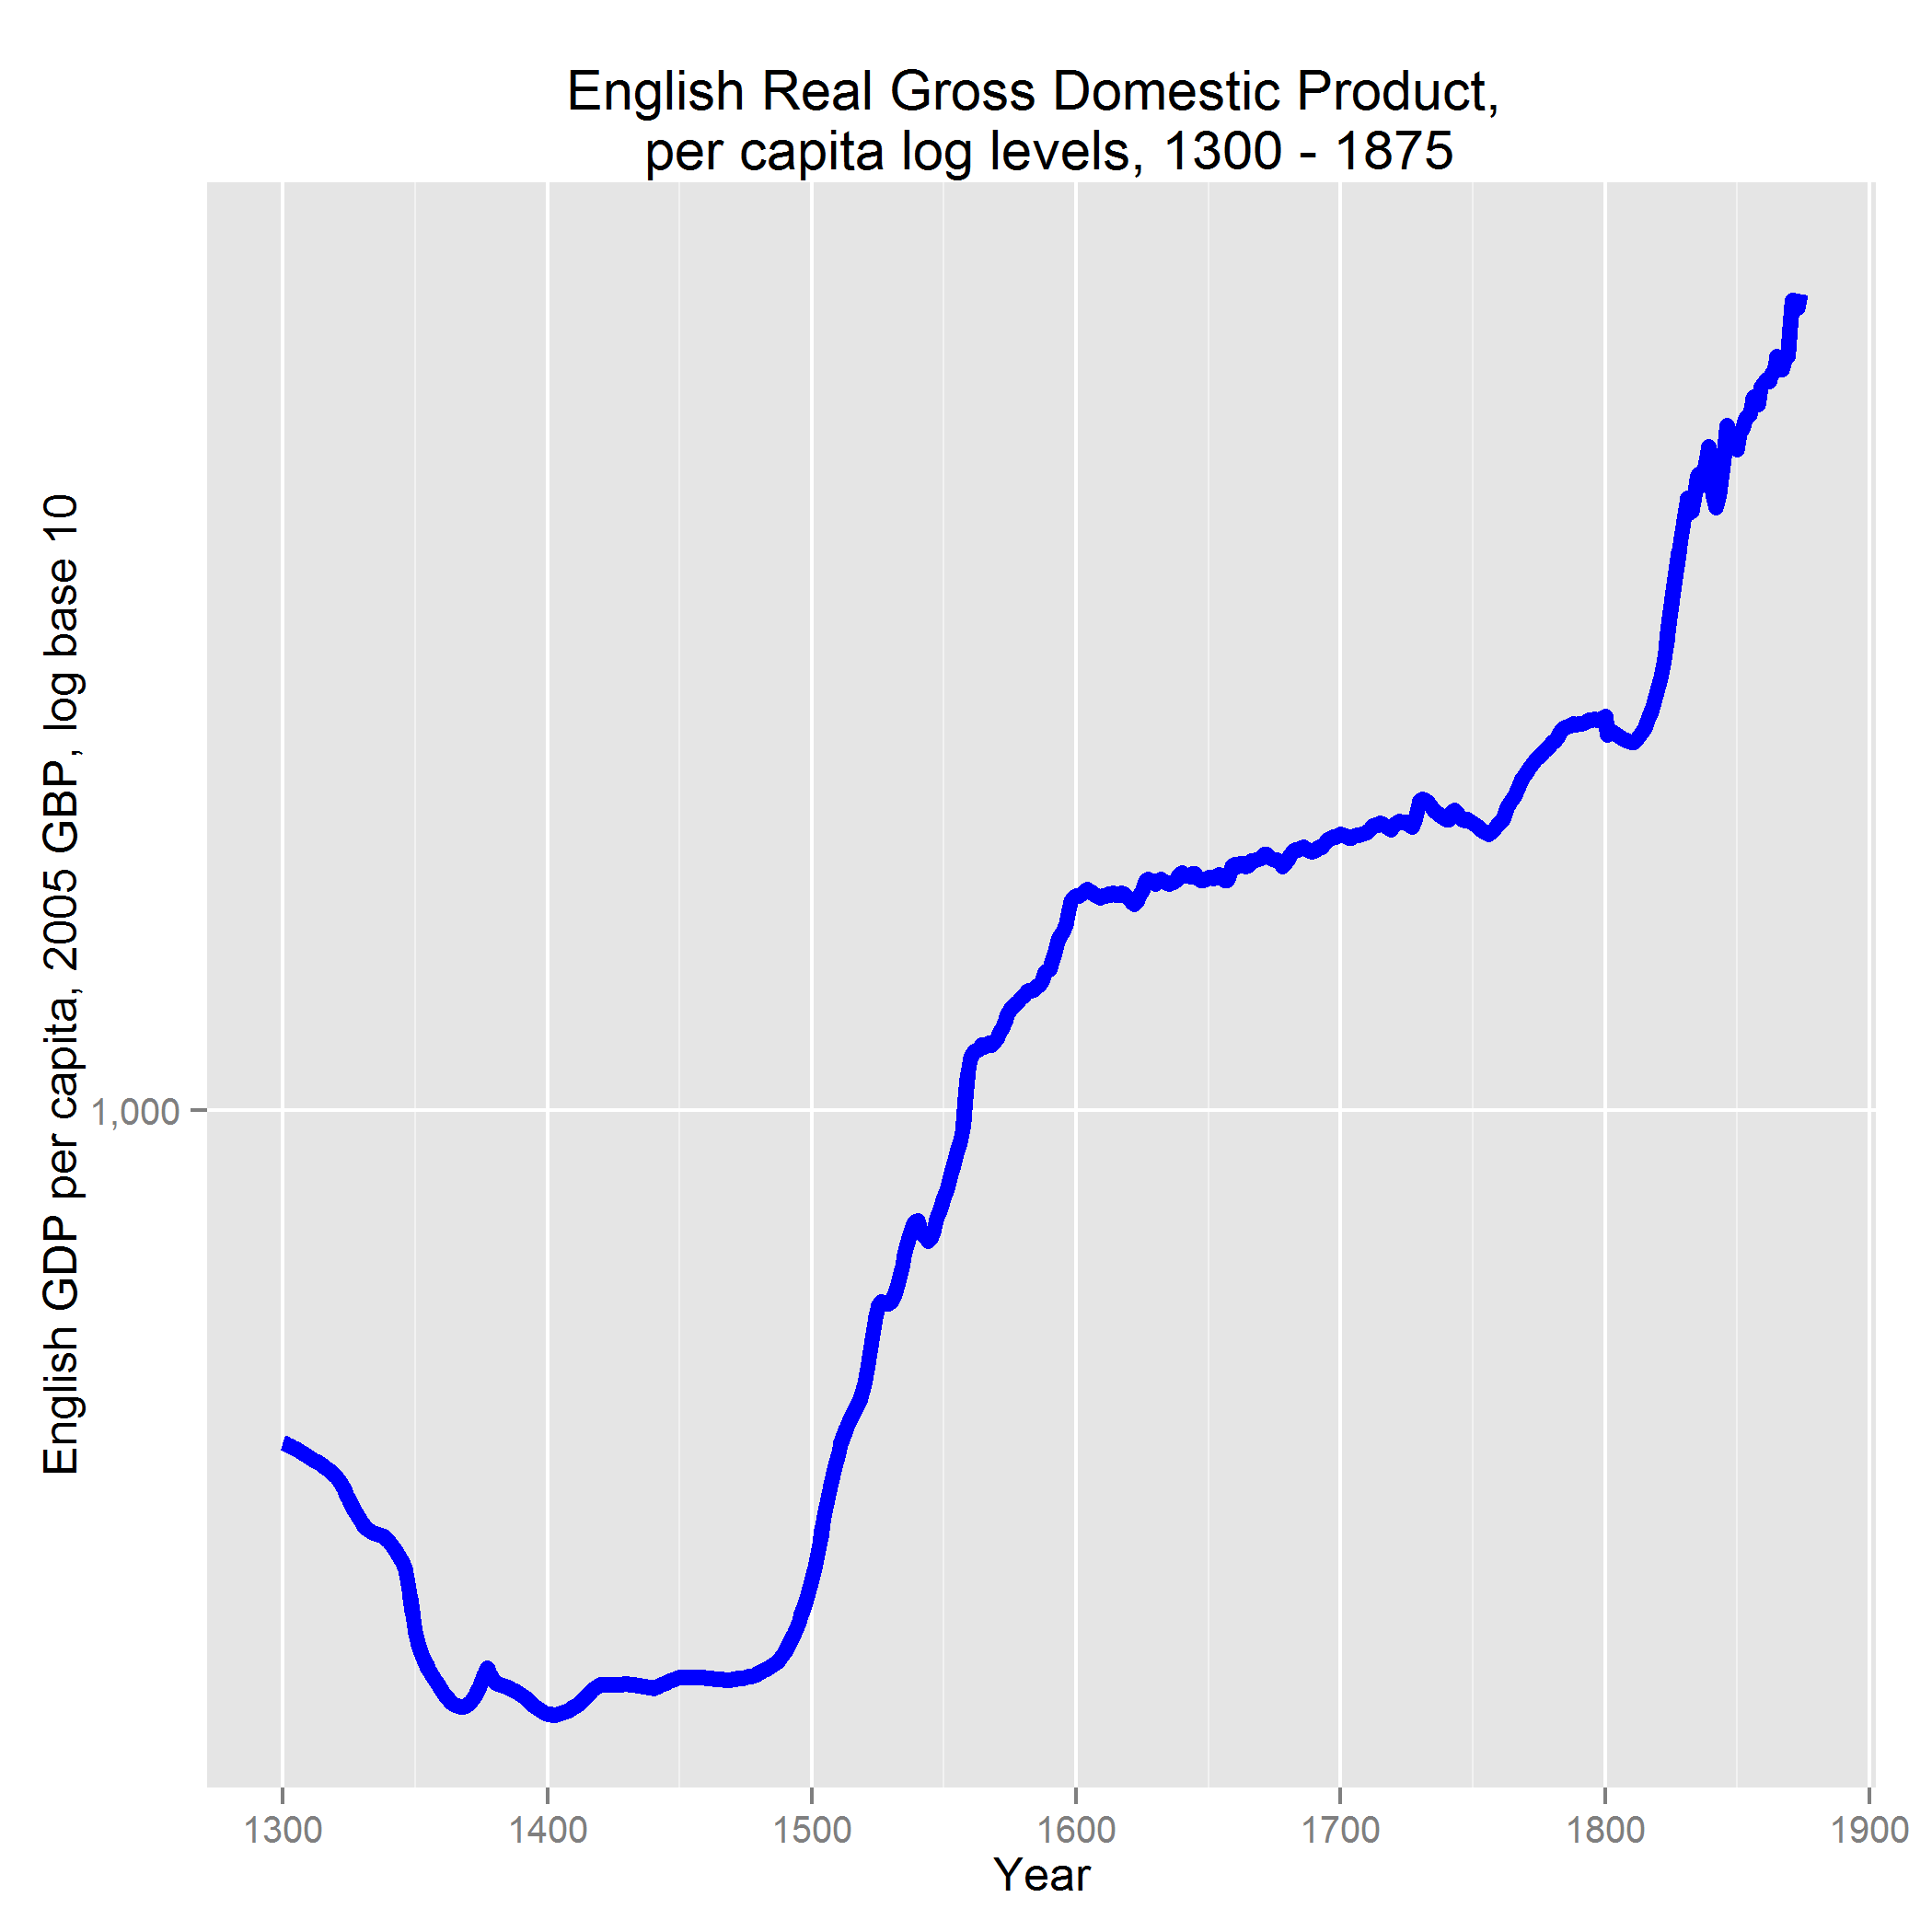
\includegraphics[width=0.55\textwidth]{gdpPopLog}}
		}
		\end{figure}
\end{frame}

\begin{frame}
		\frametitle{Structural break comparison}
\begin{figure}[p!]
%		\caption{Structural break comparison}
		\label{fig:structural}		
		\centerline{
		\mbox{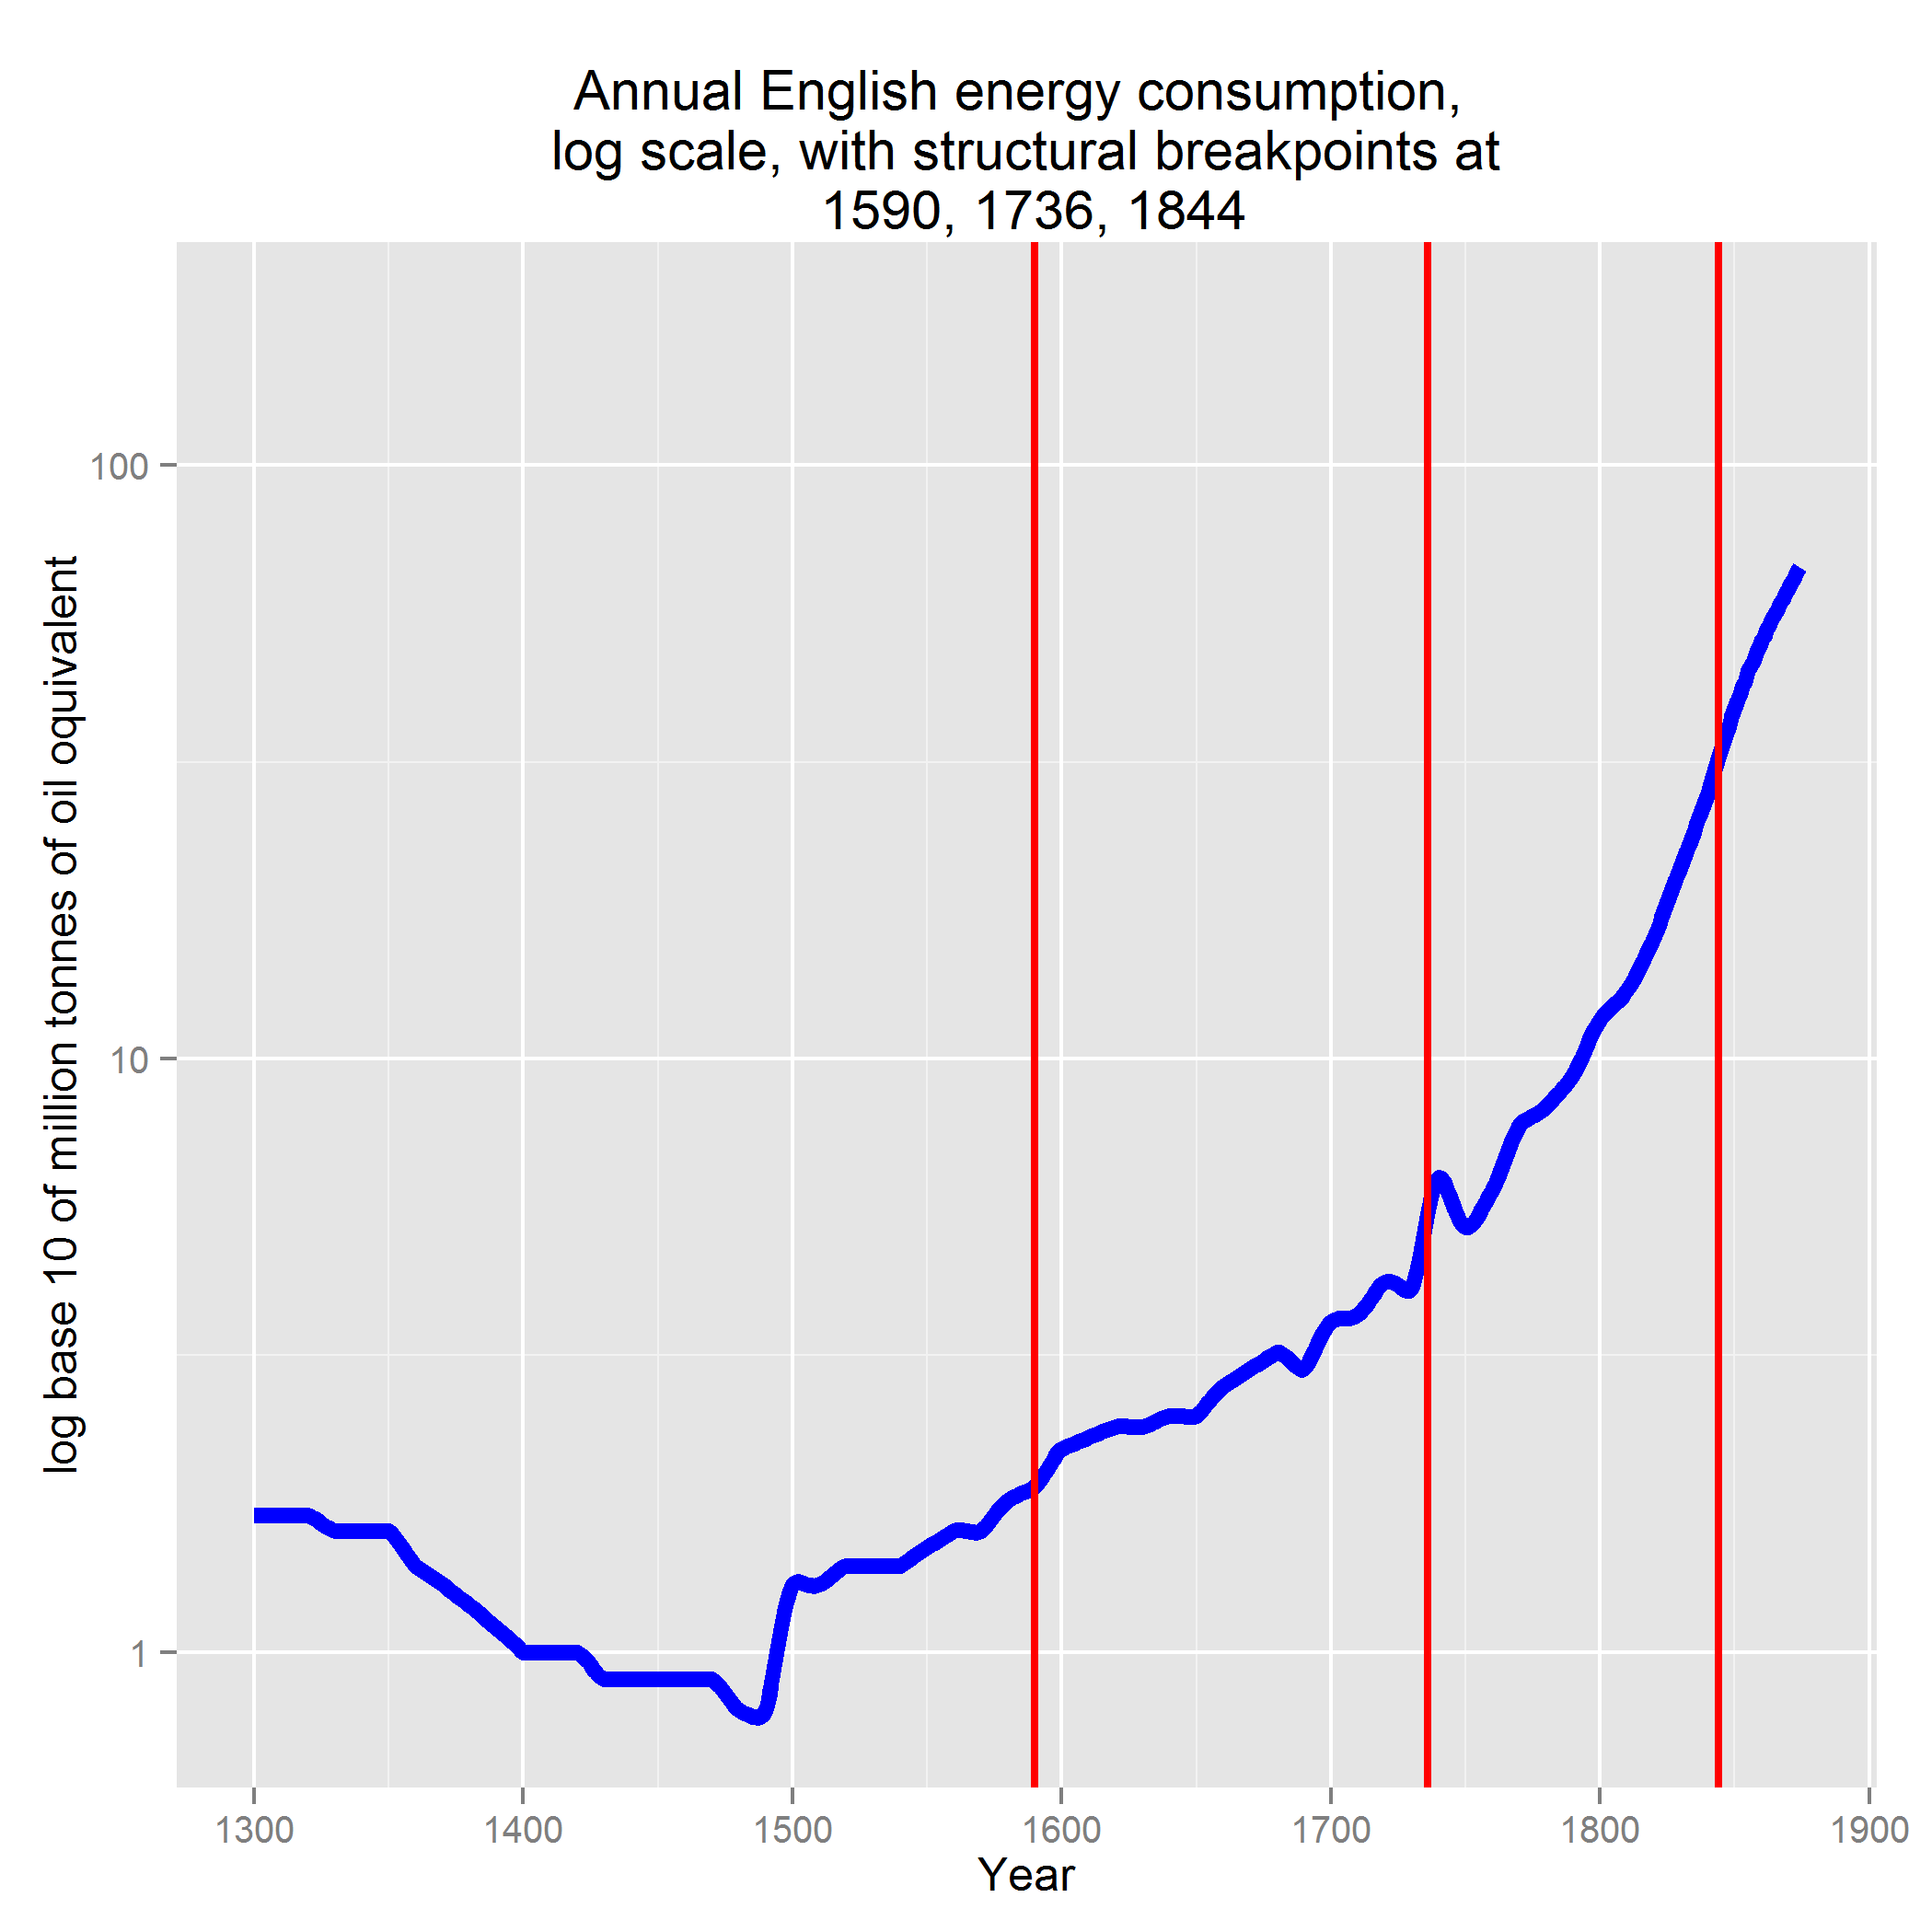
\includegraphics[width=0.39\textwidth]{energyLog1}}
		\mbox{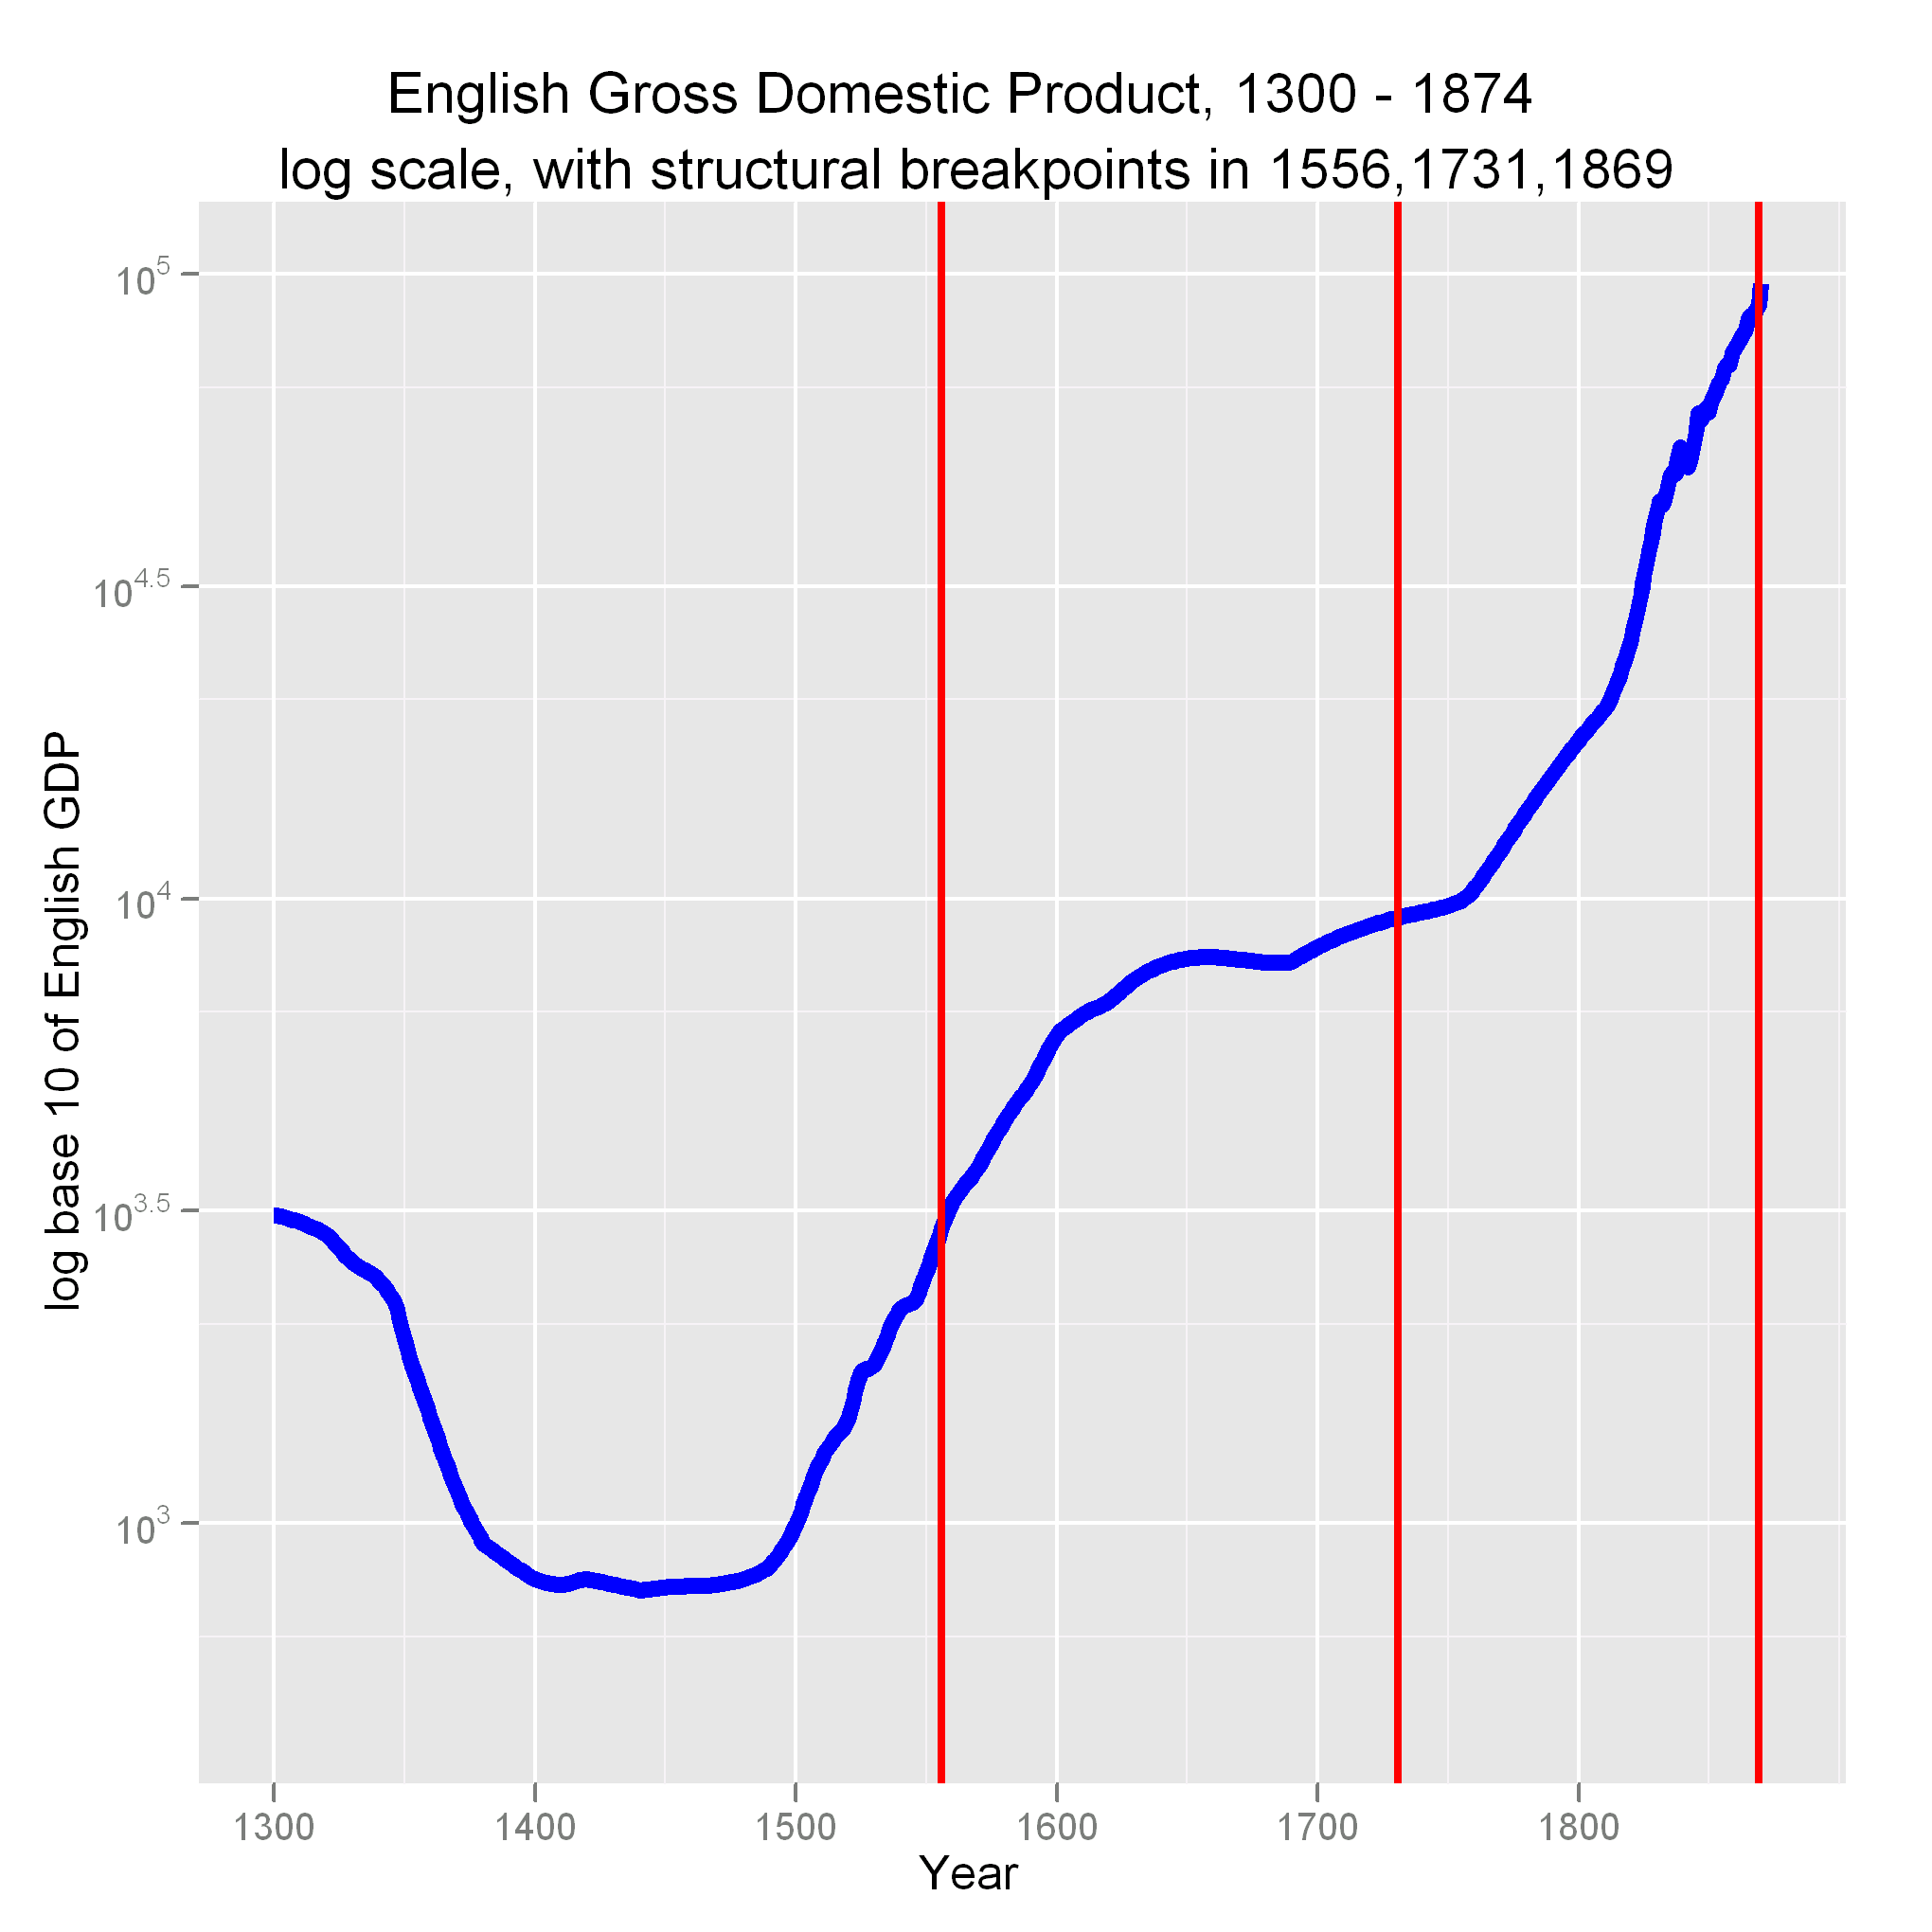
\includegraphics[width=0.39\textwidth]{gbpgdplog}}
		\mbox{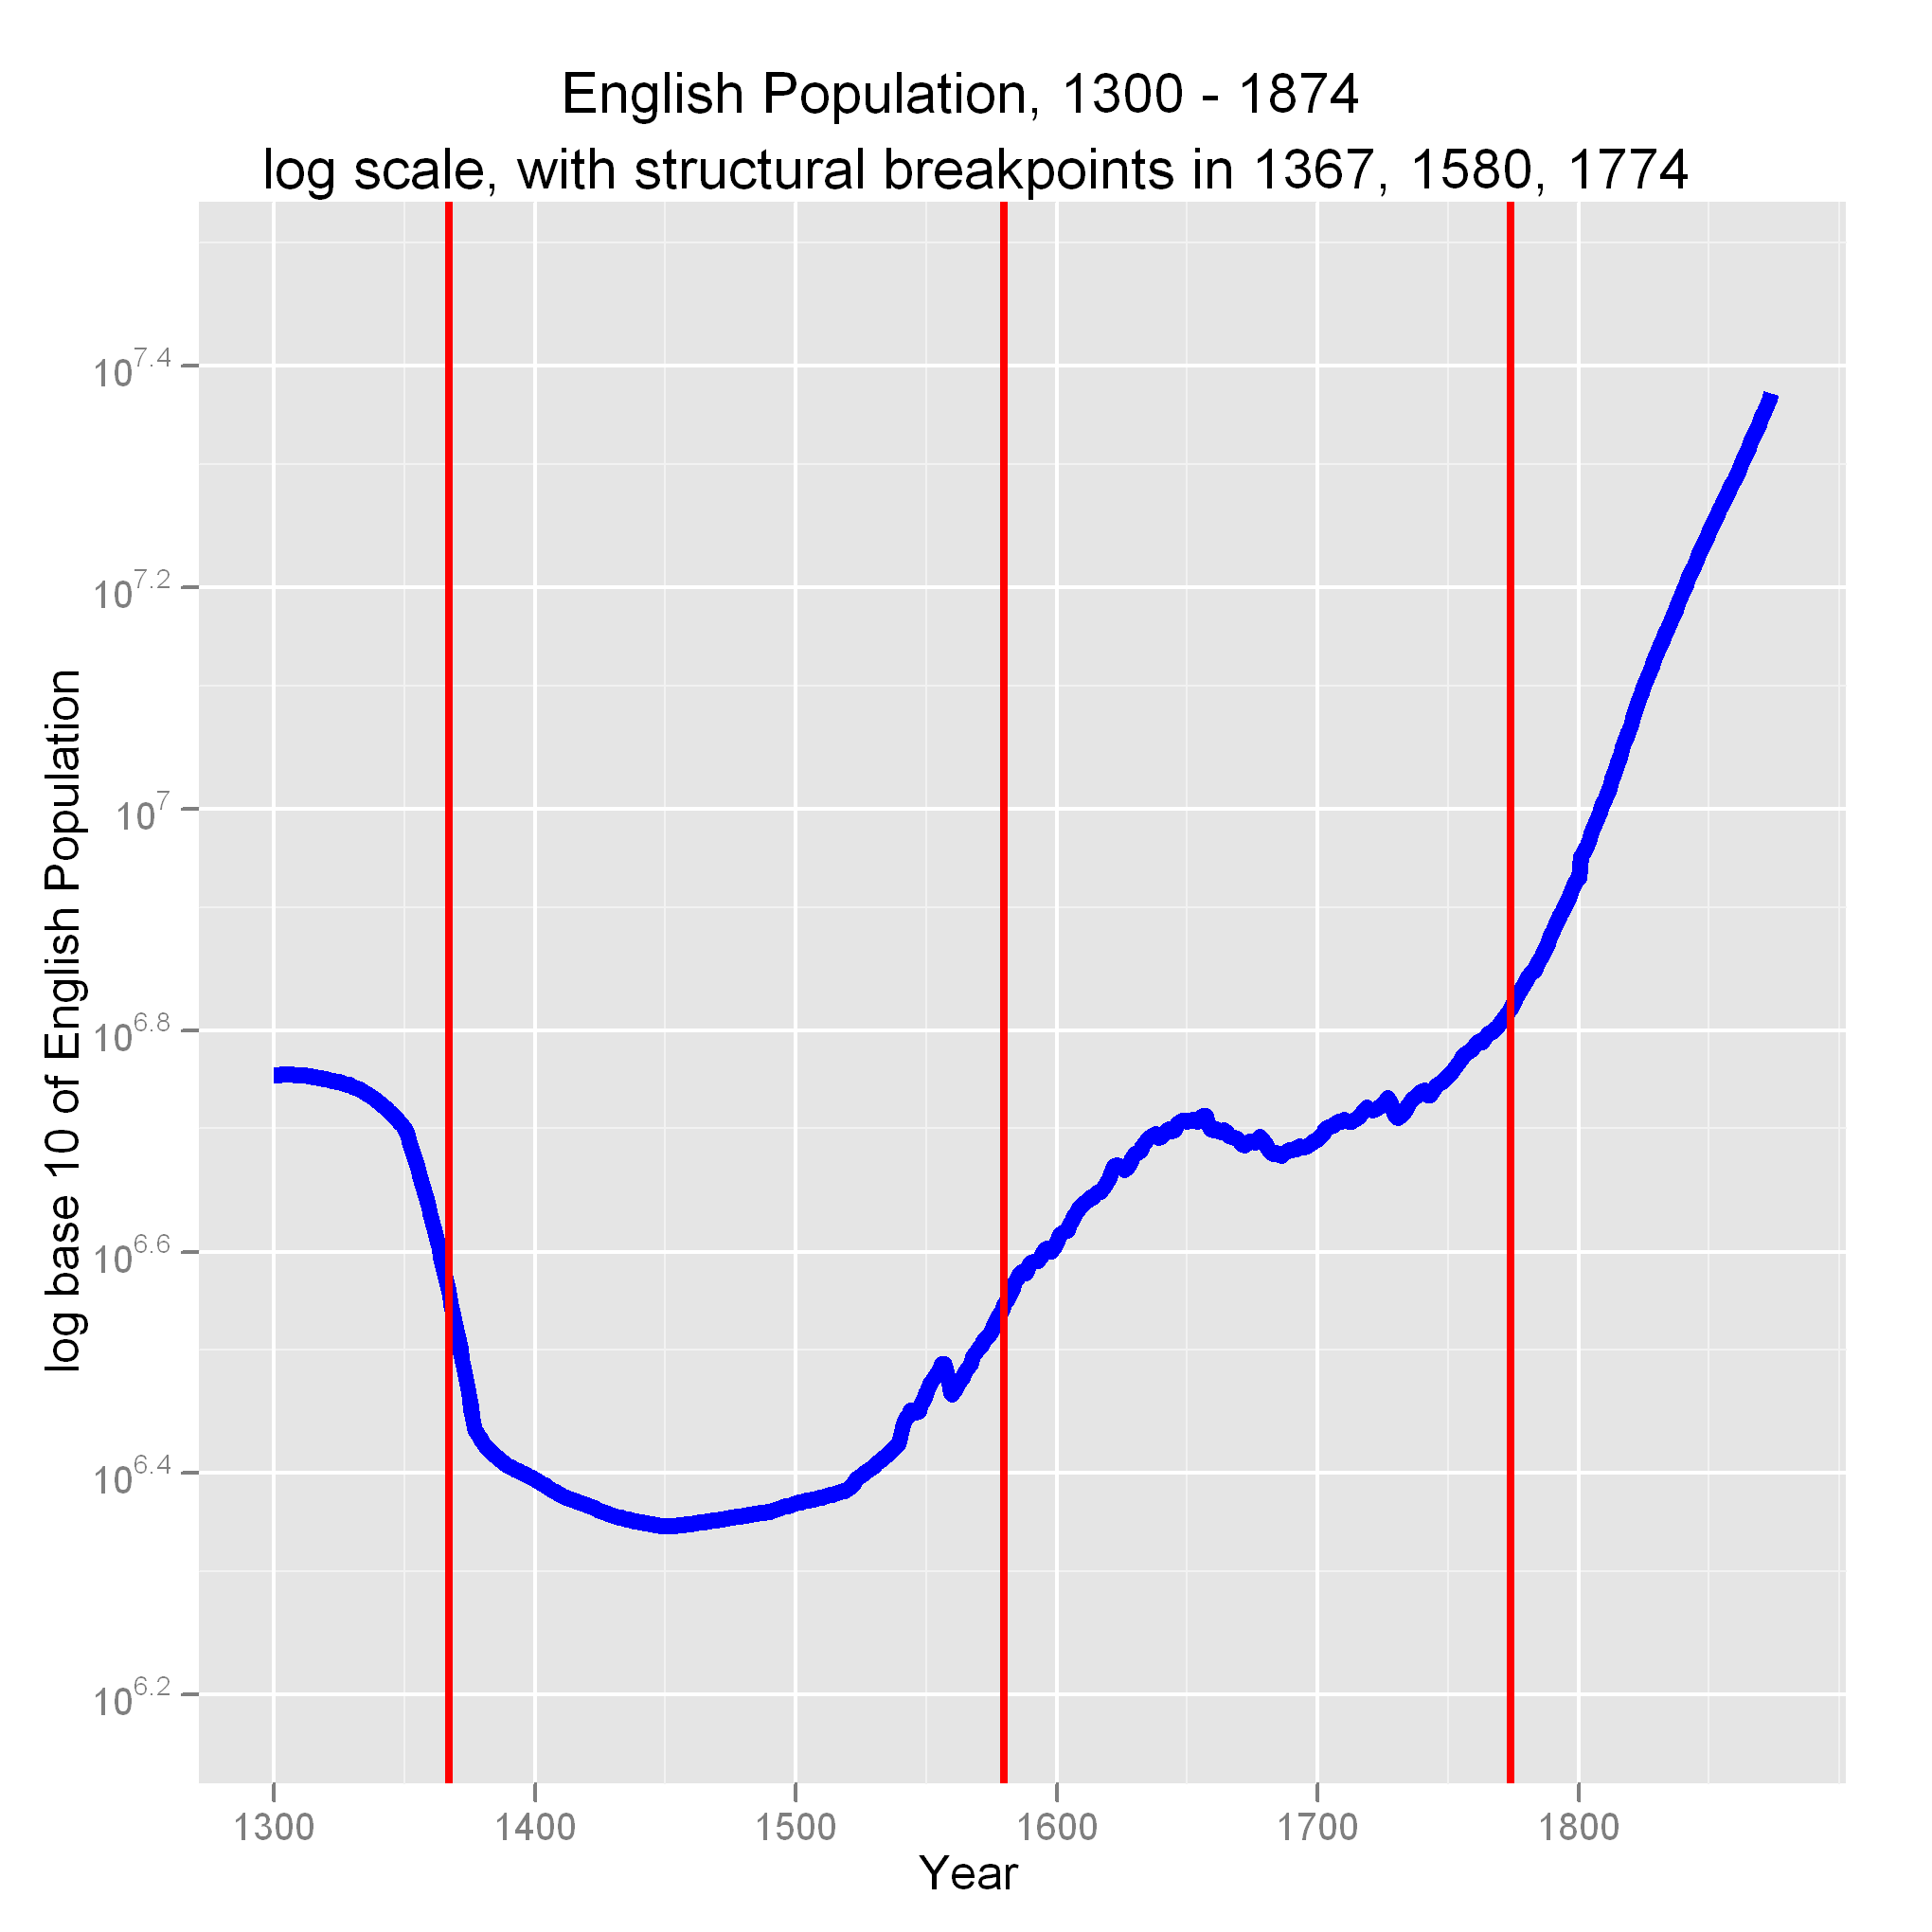
\includegraphics[width=0.39\textwidth]{popLog}}
		}
\end{figure}
\end{frame}

\begin{frame}
\frametitle{Coal and wood energy sources\\\textit{Source:} Pearson \& Fouquet}
\begin{figure}[p!]
\center
%\caption{Coal and wood energy sources\\\textit{Source:} Pearson \& Fouquet}
\label{fig:woodCoal}
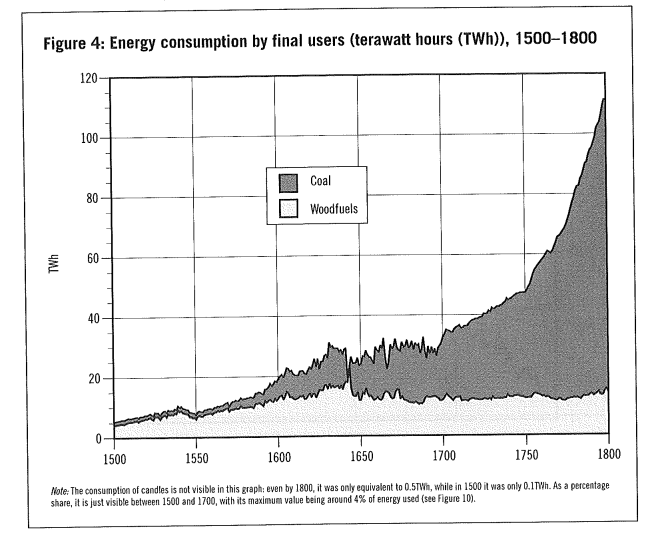
\includegraphics[height=0.8\textheight]{woodCoal.png}
\end{figure}
\end{frame}

\begin{frame}
\frametitle{Energy consumption vs. standarized GDP}
\begin{figure}[p!]
\center
%\caption{Energy consumption vs. standarized GDP}
\label{fig:energyVsGdp}
		\centerline{
		\mbox{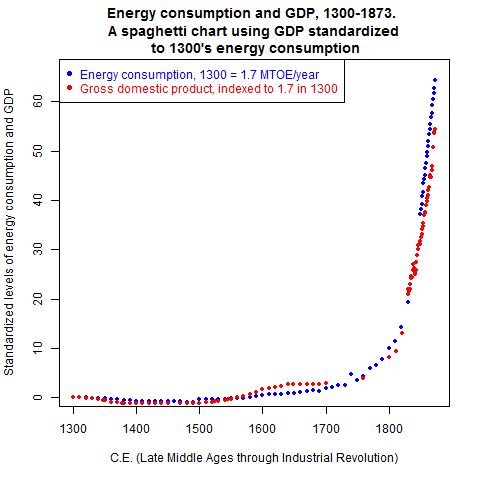
\includegraphics[width=0.55\textwidth]{energyVsGdp}}
		\mbox{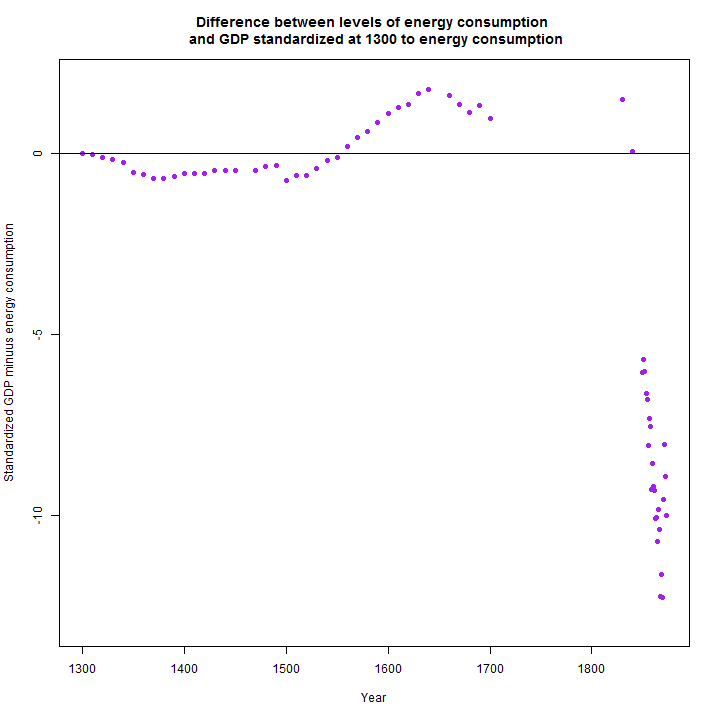
\includegraphics[width=0.55\textwidth]{energyVsGdpDiff}}
		}
\end{figure}
\end{frame}

\begin{frame}
\frametitle{Scatterplot of energy consumption vs. GDP}
\begin{figure}[p!]
\center
%\caption{Scatterplot of energy consumption vs. GDP}
\label{fig:scatterplot}
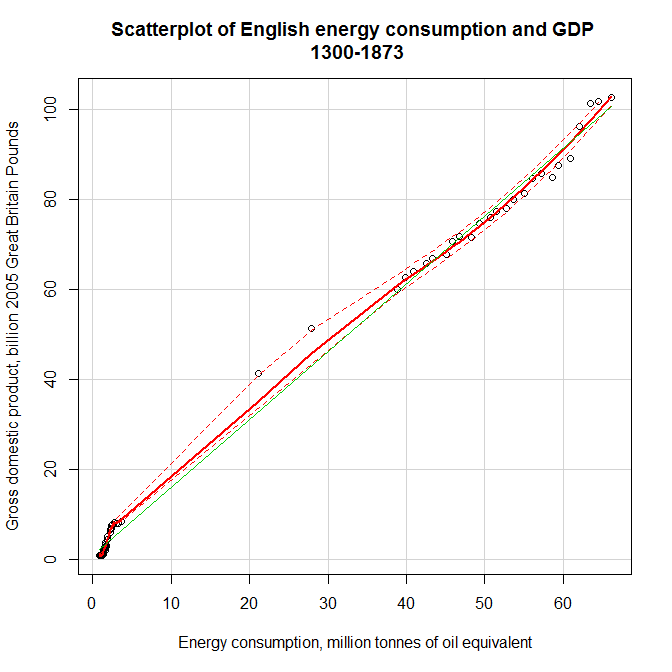
\includegraphics[height=0.8\textheight]{scatterplot.png}
\end{figure}
No ``Solow'' residual
\end{frame}

\begin{frame}
\frametitle{Granger tests of energy/GDP dynamics}
\scriptsize{
\begin{table}[p!]
%\caption{Granger tests of energy/GDP dynamics}
\label{tbl:grangerEnergyGdp}
\begin{tabular}{lrrl}
Era&Energy $\sim$ GDP Pr($>$F)& GDP $\sim$ Energy Pr($>$F)&AS/AD regime\\
\hline \hline
1300 -- 1500&0.0106&0.0003&EMP \footnote{European marriage pattern (Hajnal)}, Black Death: \\&&&increasing wages, \\
&&&family income\\
1500 -- 1600&0.1939&0.6126&Positive demand shock\\
1600 -- 1750&0.3529&0.5185&Energy supply constraint\\
1750 -- 1873&0.0024&0.1100&Positive supply shock:\\&&&``virtuous'' macro \\
&&&feedback cycle\\
\hline
1300 -- 1873& 0.0002& 0.0361&Total study period\\
\end{tabular}
\end{table}
}
\end{frame}

\begin{frame}
		\frametitle{Aggregate Supply - Aggregate Demand \\ Four energy/GDP regimes}
\begin{figure}[p!]
%		\caption{Aggregate Supply - Aggregate Demand \\ Four energy/GDP regimes}
		\label{fig:asad}		
		\centerline{
		\mbox{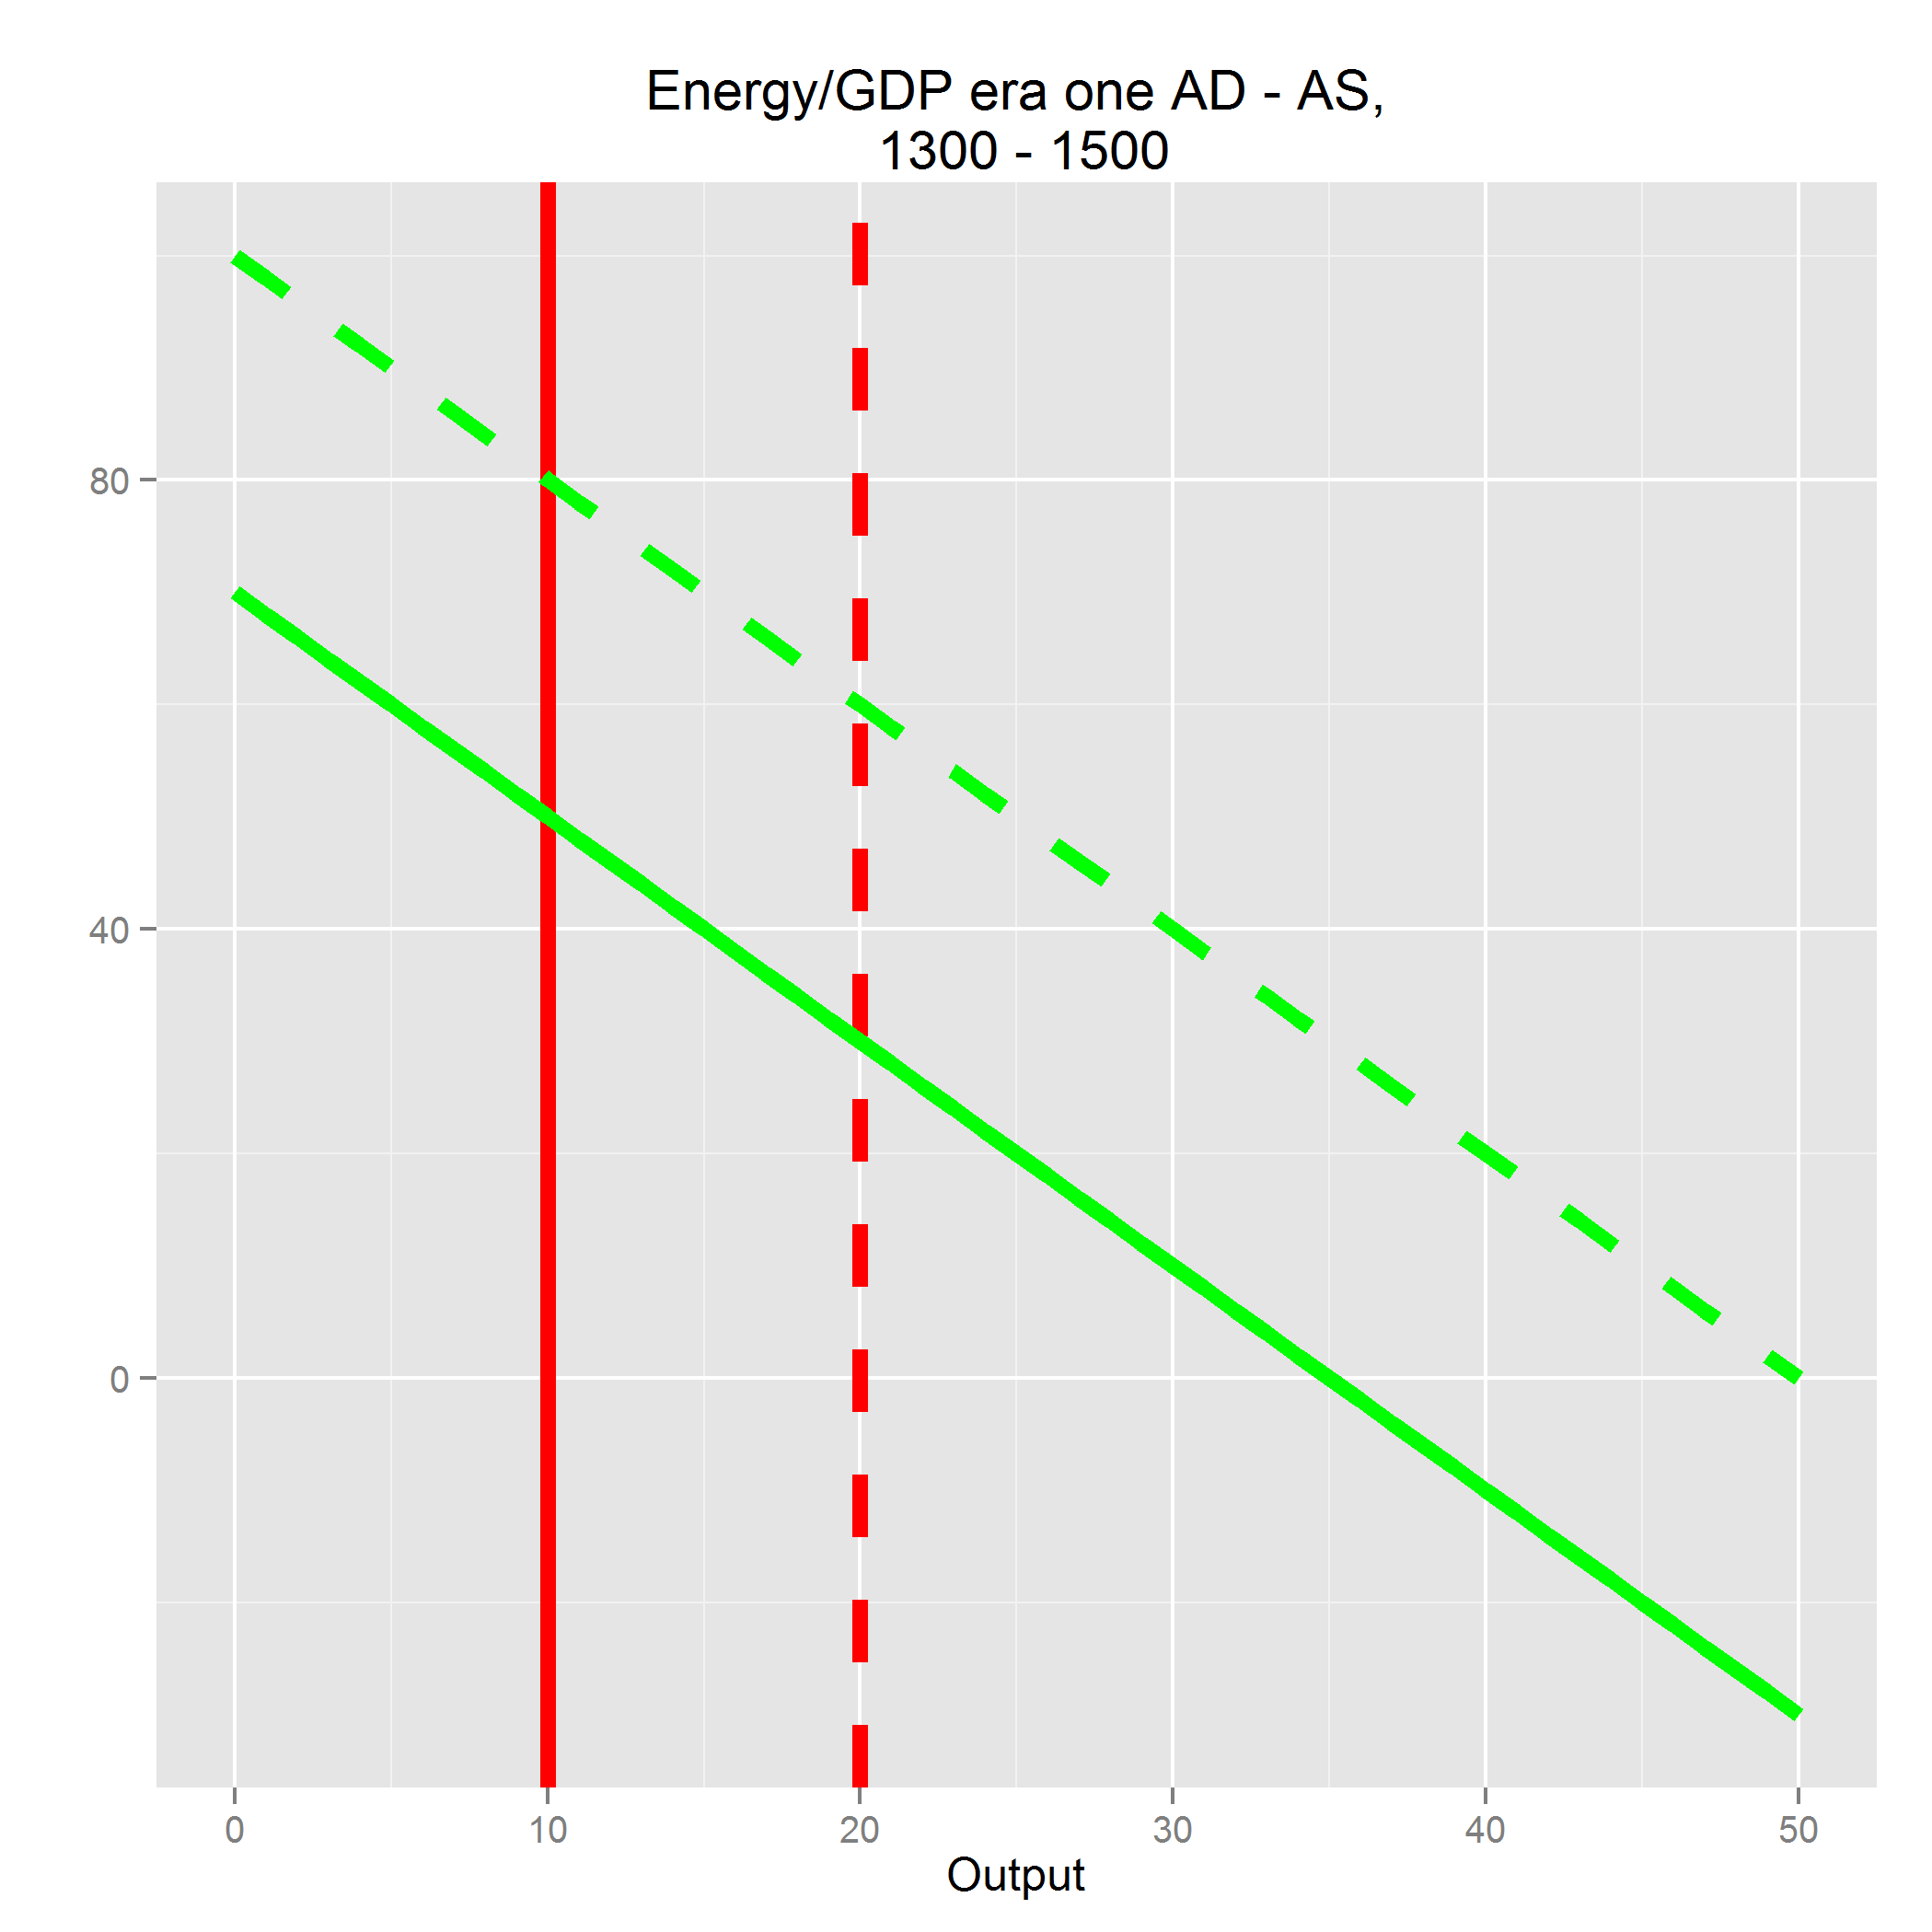
\includegraphics[height=0.35\textheight]{era1}}
		\mbox{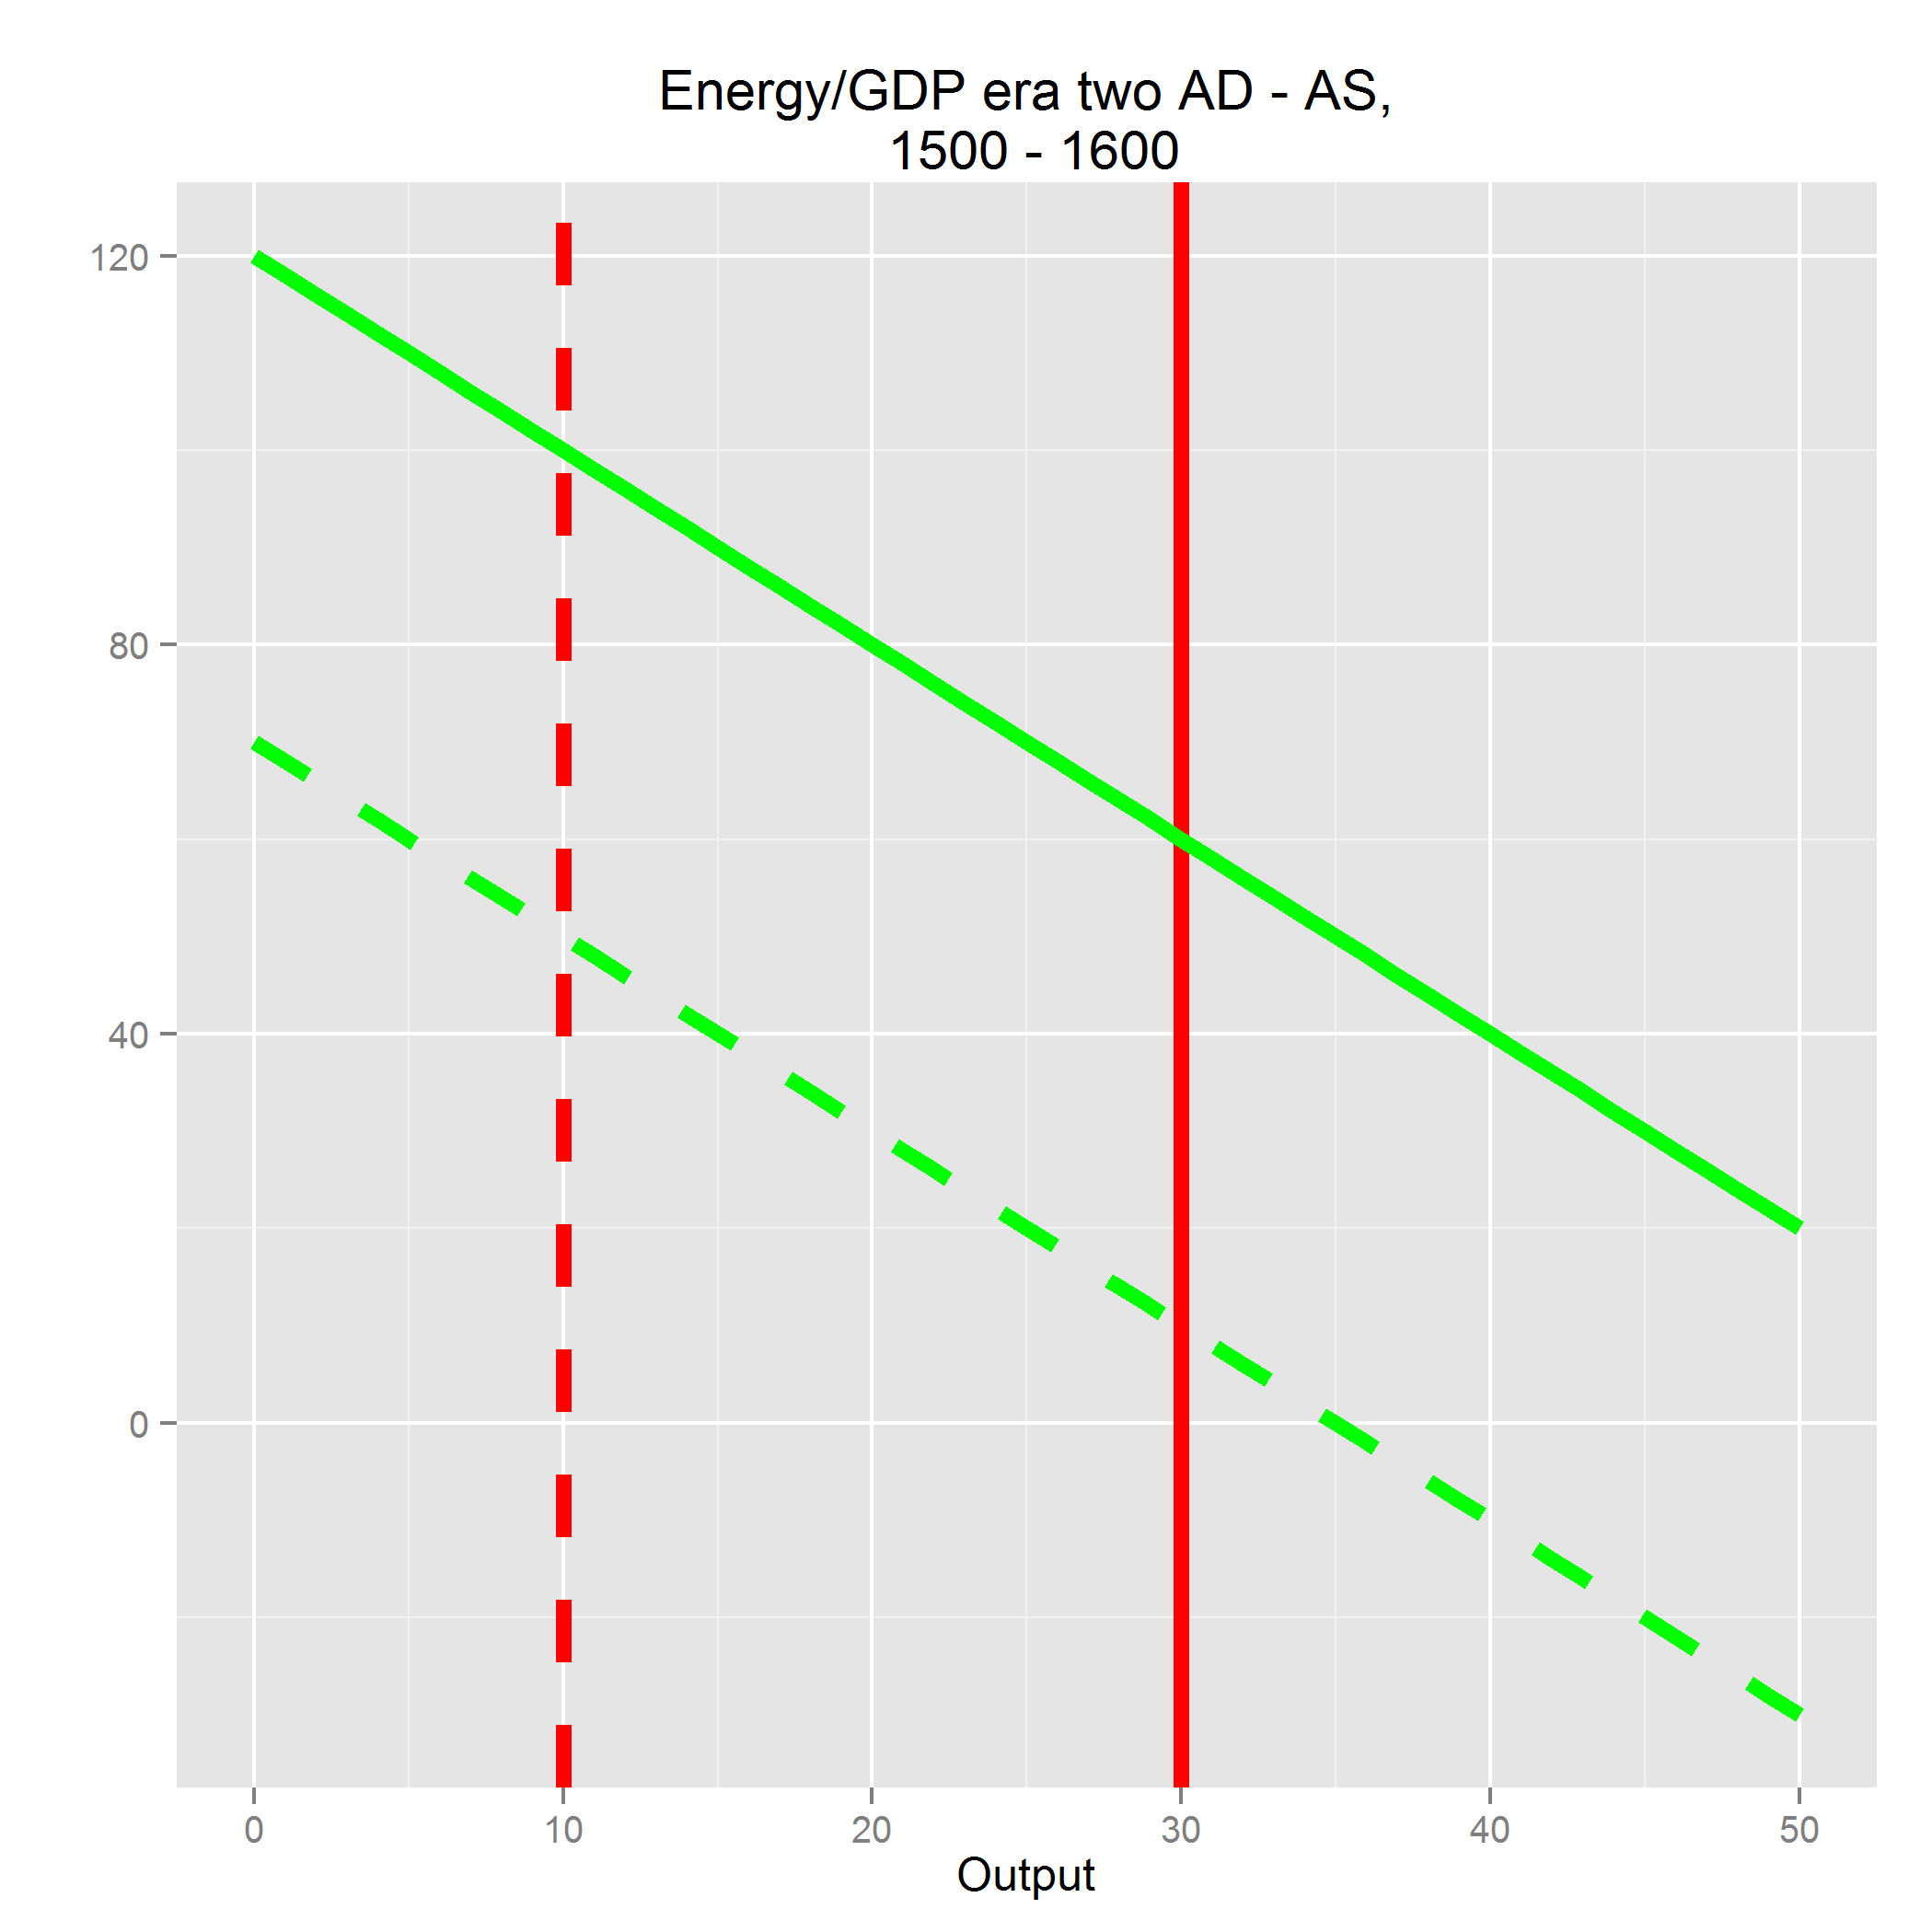
\includegraphics[height=0.35\textheight]{era2}}
		}
		\end{figure}
\begin{figure}[p!]
%		\caption{Aggregate Supply - Aggregate Demand \\ Four energy/GDP regimes}
		\label{fig:asad}		
		\centerline{
		\mbox{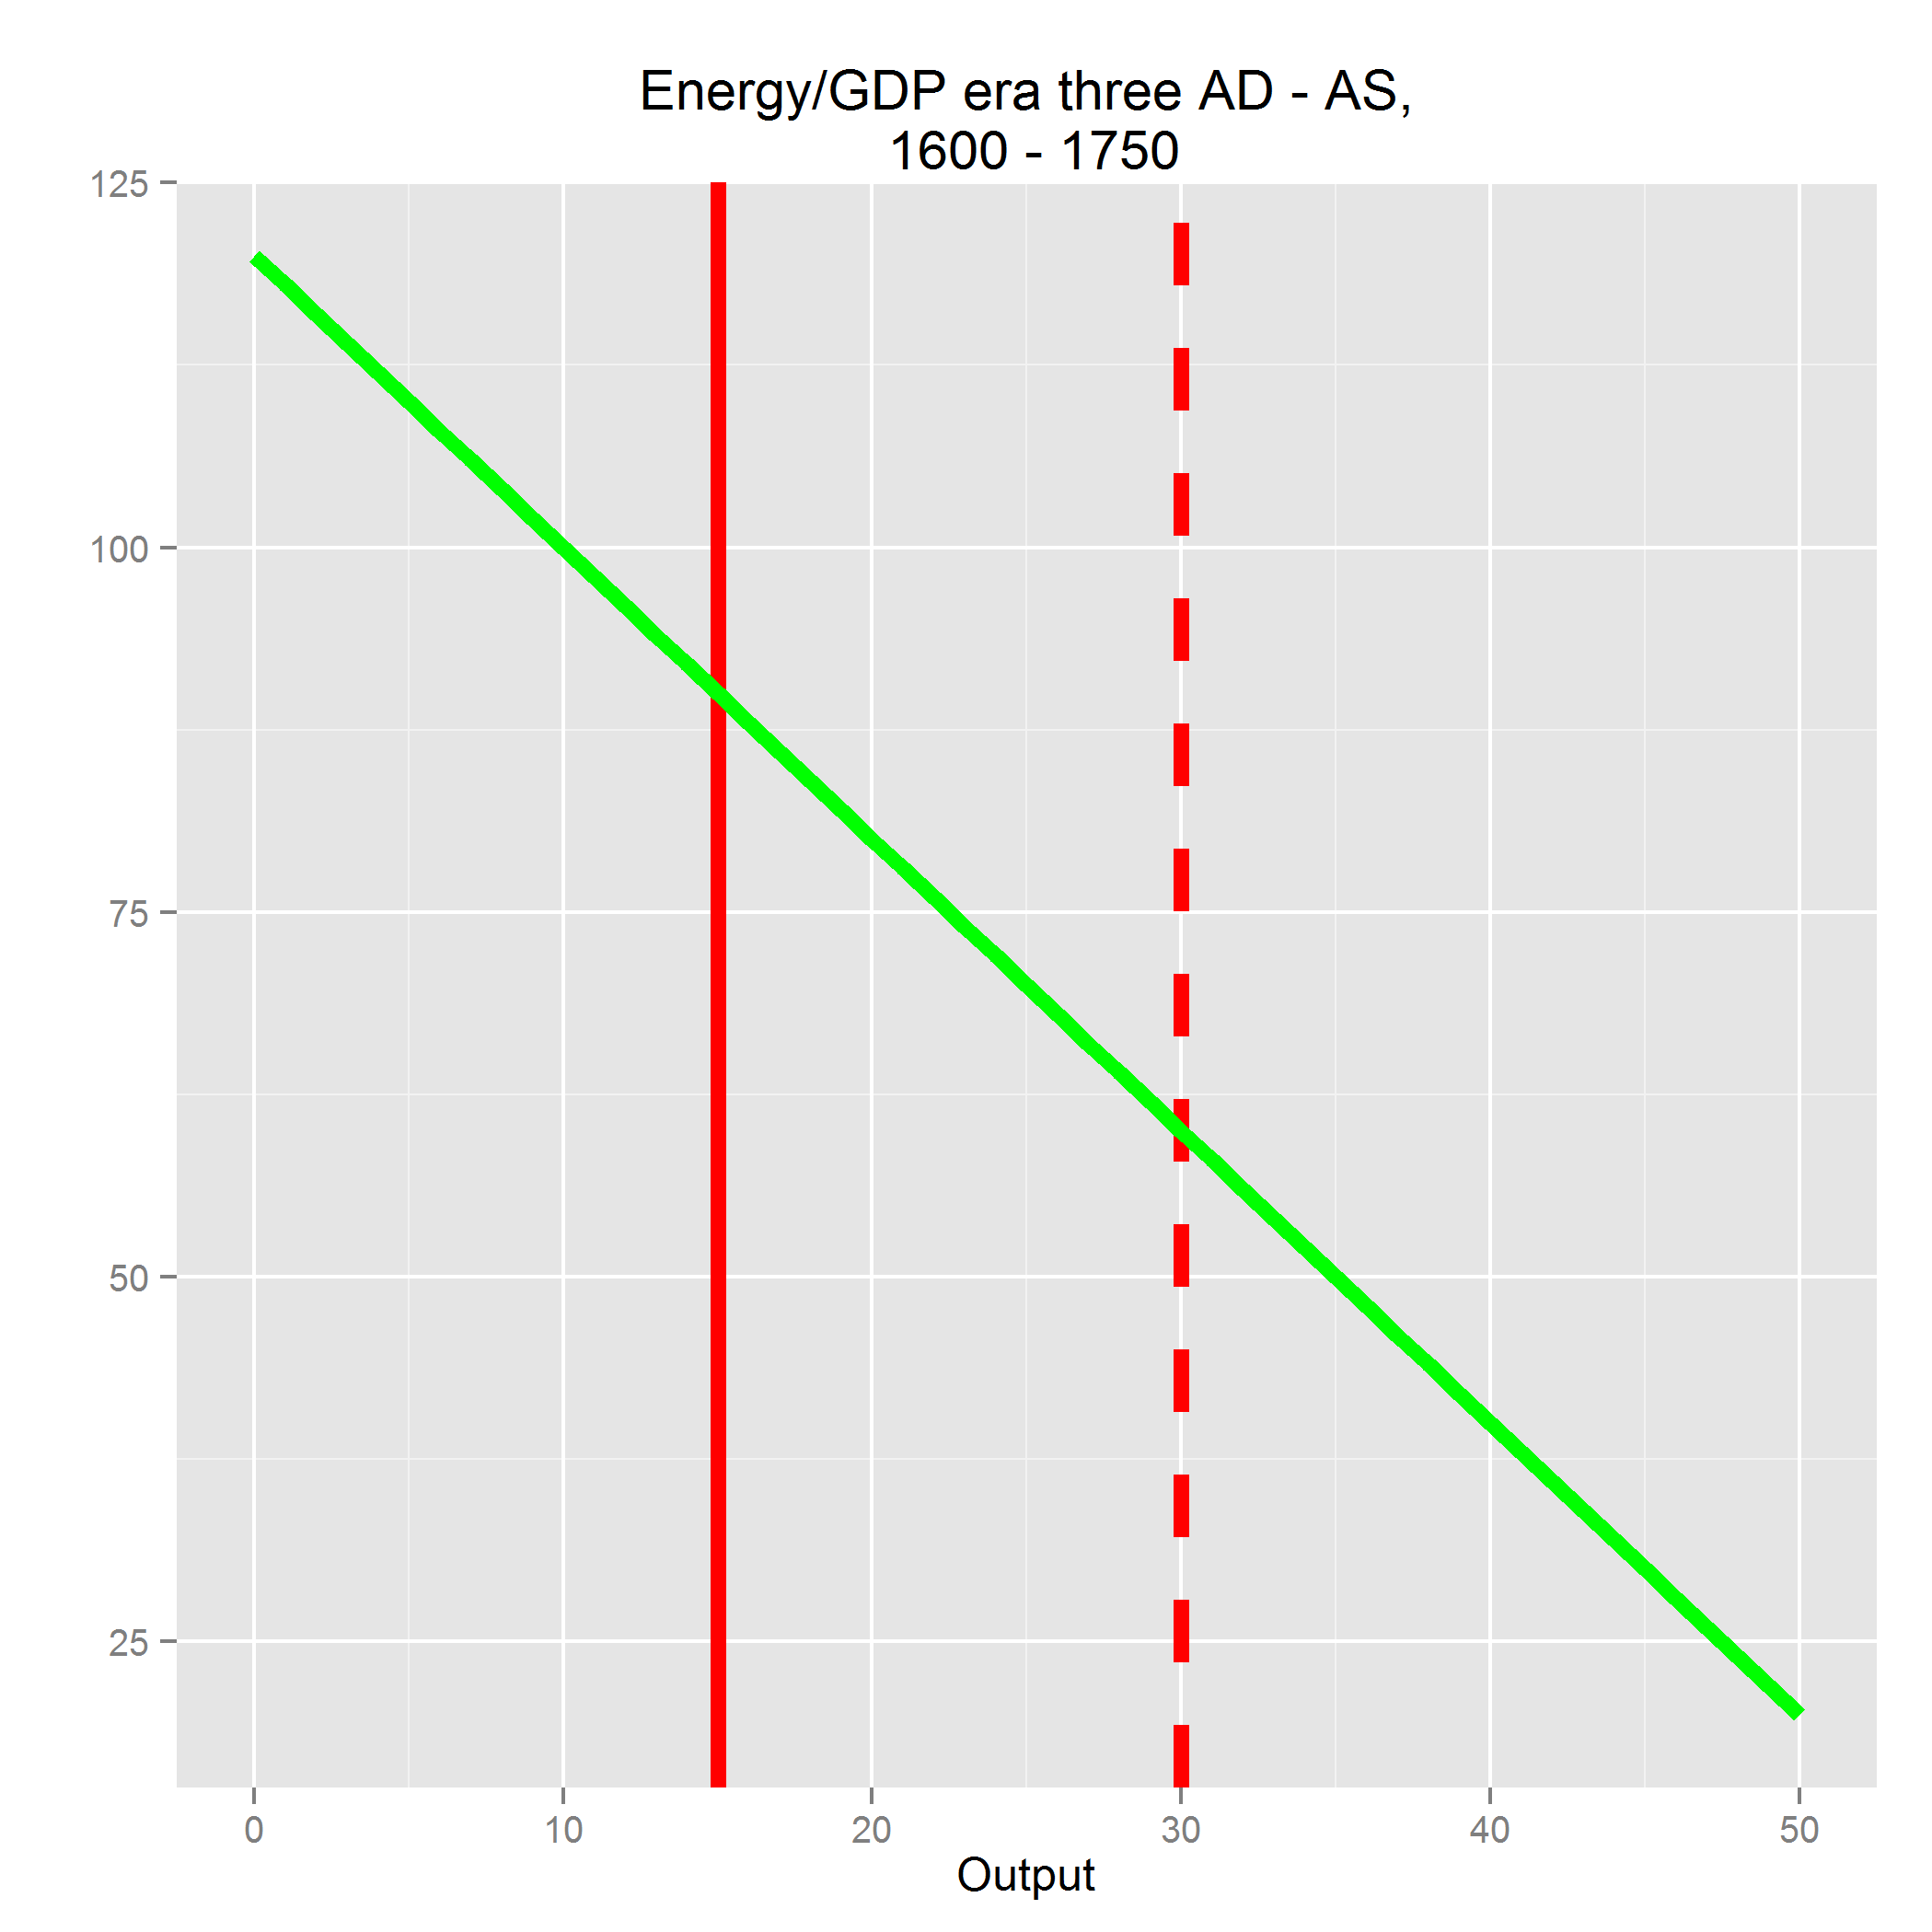
\includegraphics[height=0.35\textheight]{era3}}
		\mbox{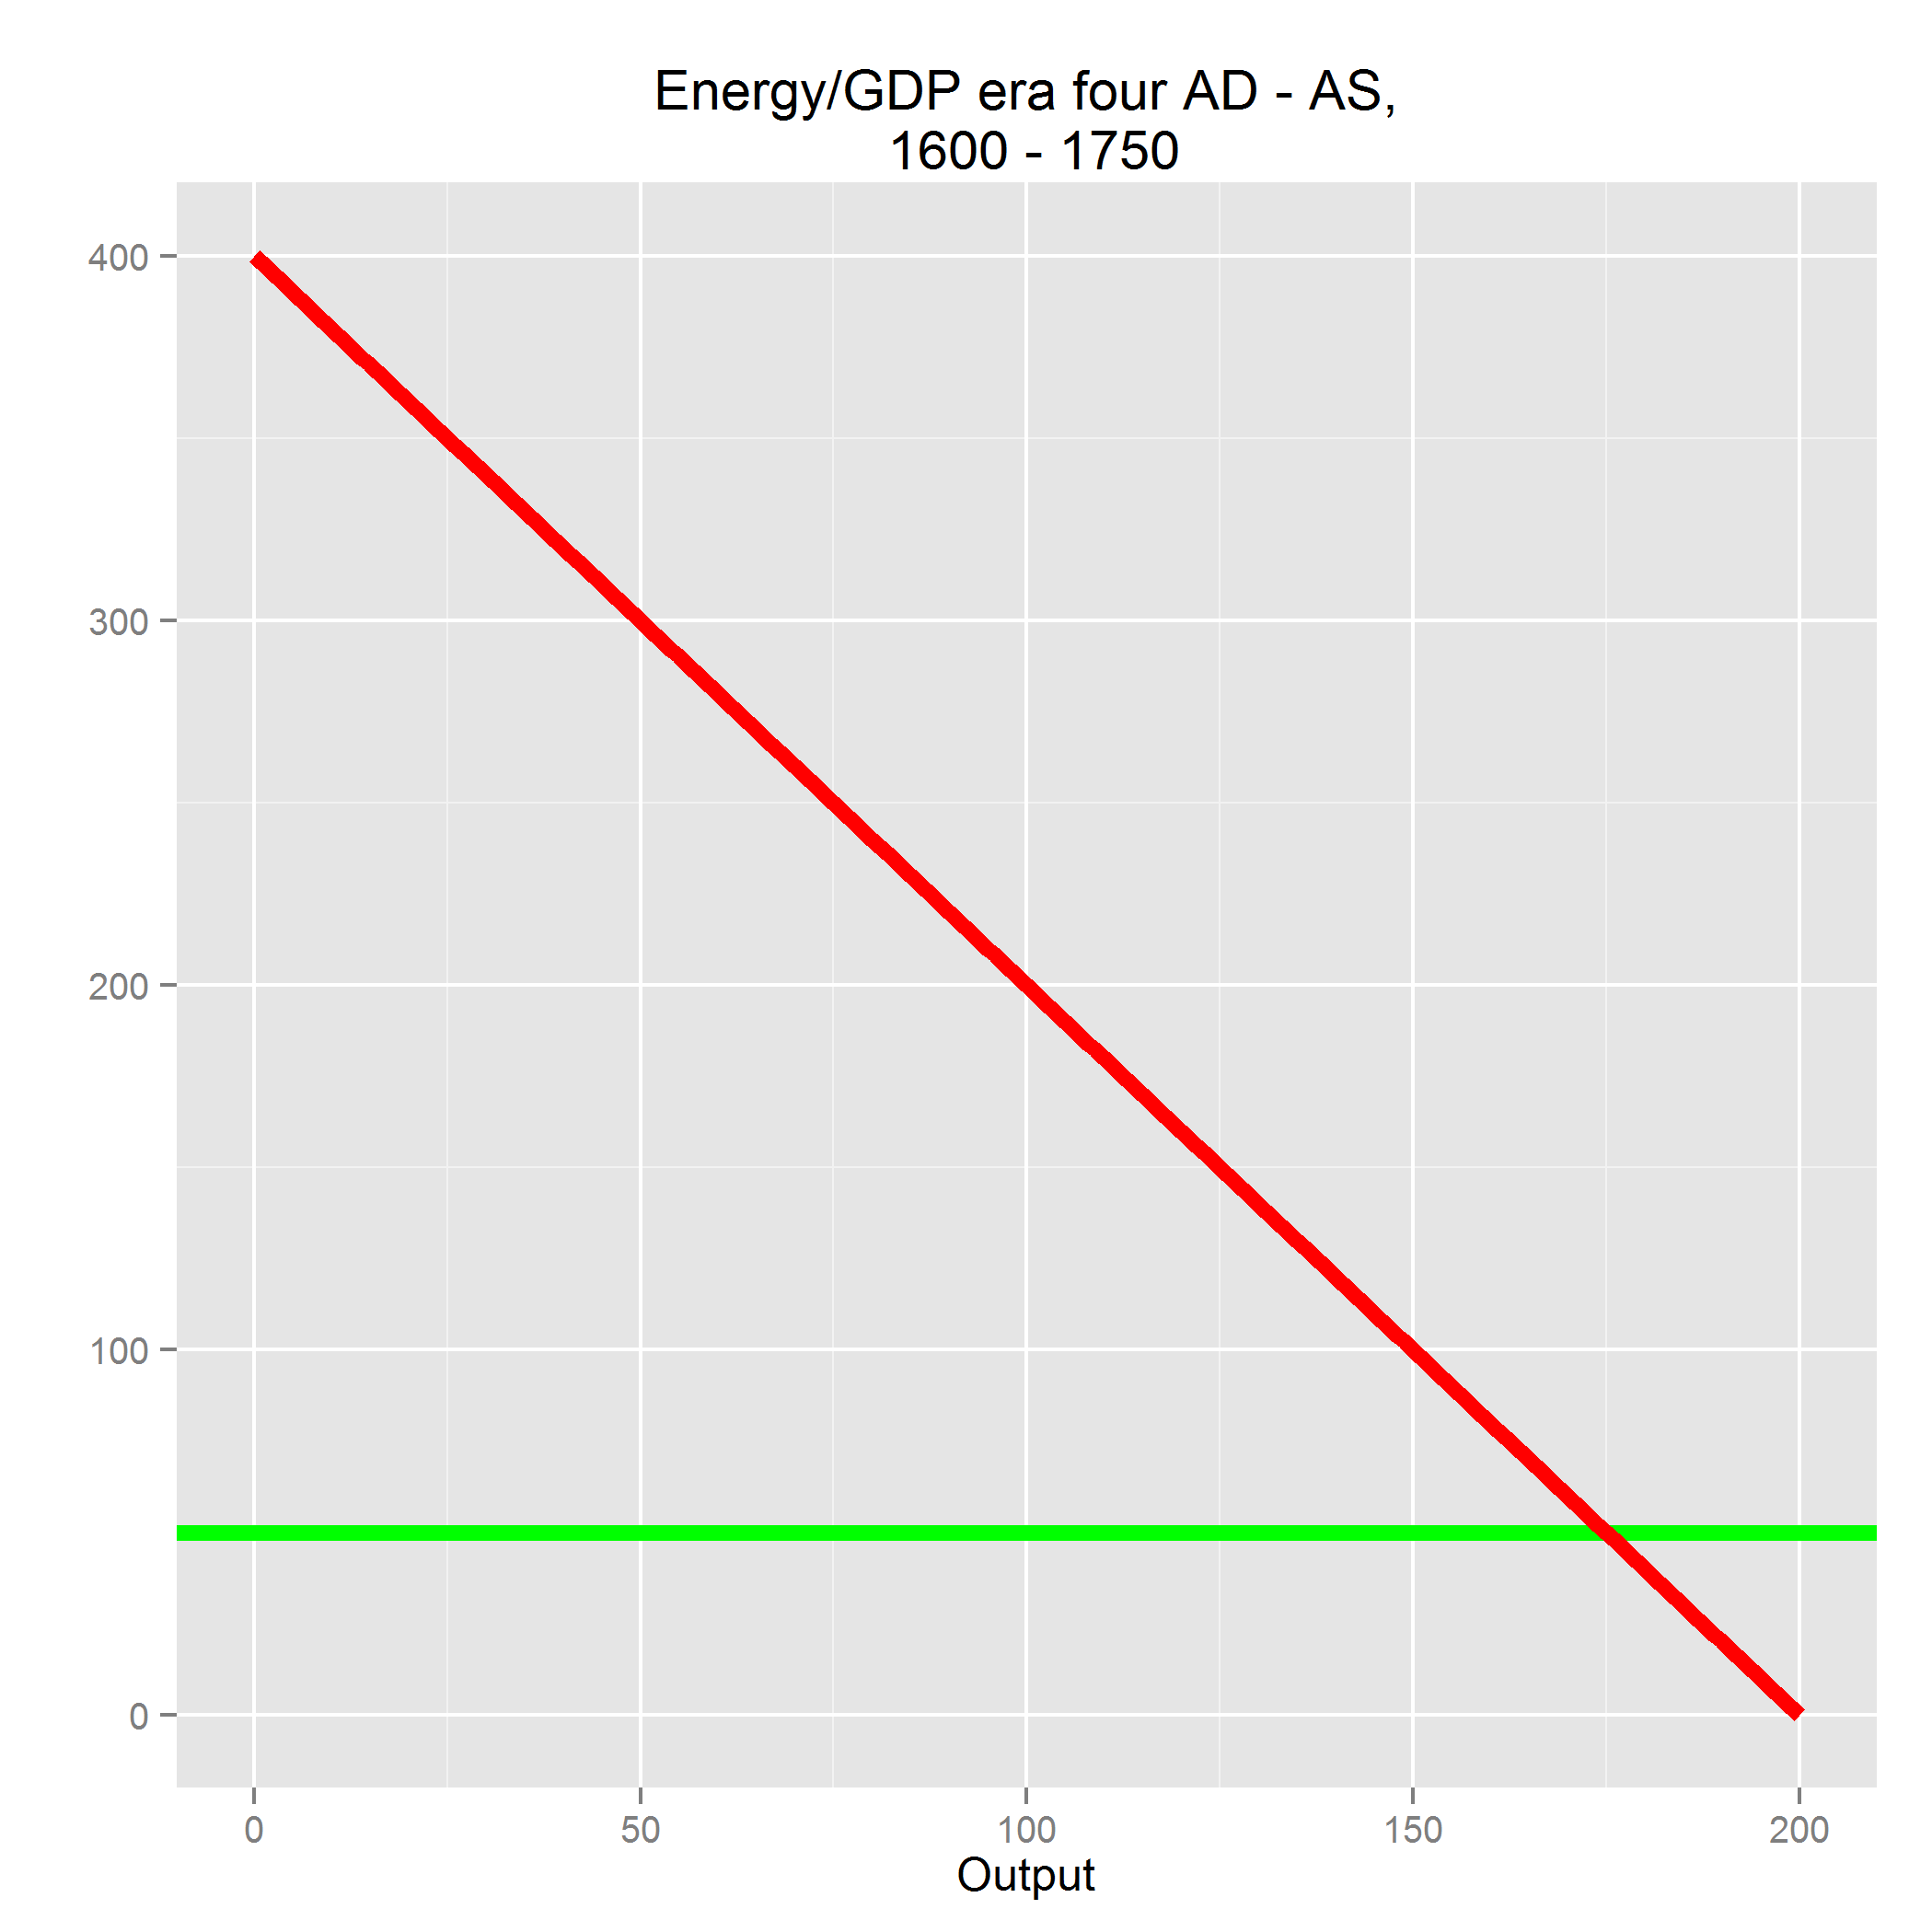
\includegraphics[height=0.35\textheight]{era4}}				
		}
		\end{figure}
\end{frame}


\begin{frame}
		\frametitle{Desagulier manuscript}
\begin{figure}[p!]
%		\caption{Desagulier manuscript}
		\label{fig:desagulier}		
		\center
%		\mbox{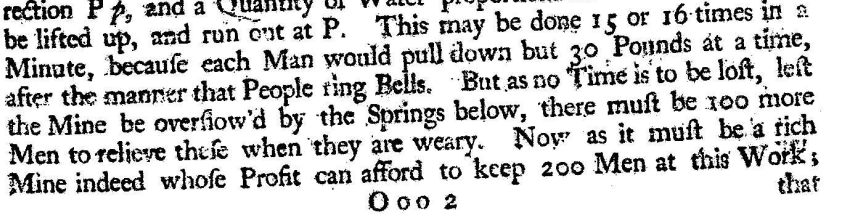
\includegraphics[width=0.95\textwidth]{desagulier1}}\\
%		\mbox{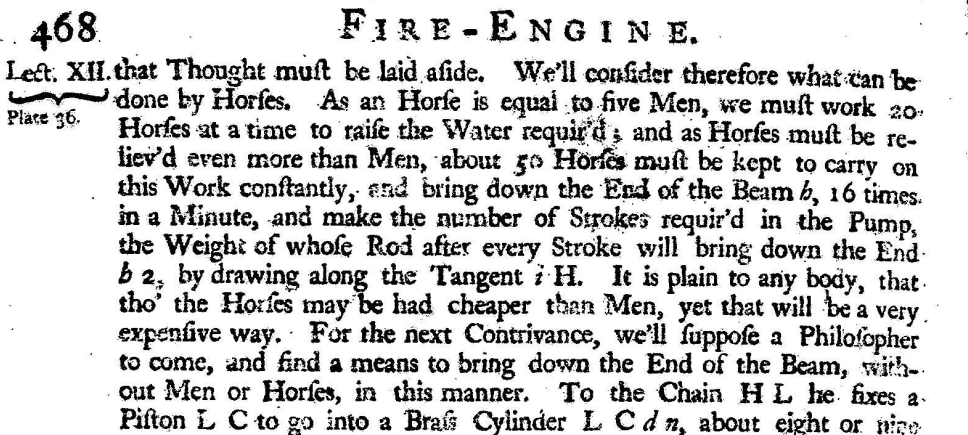
\includegraphics[width=0.95\textwidth]{desagulier2}}
		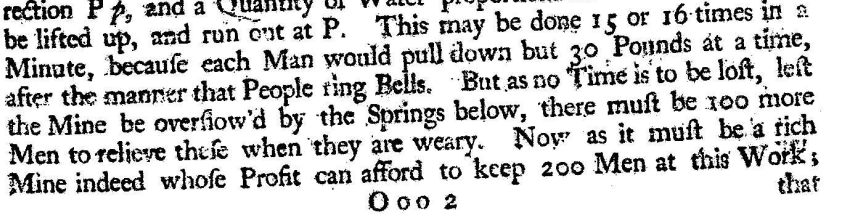
\includegraphics[width=0.95\textwidth]{desagulier1}\\
		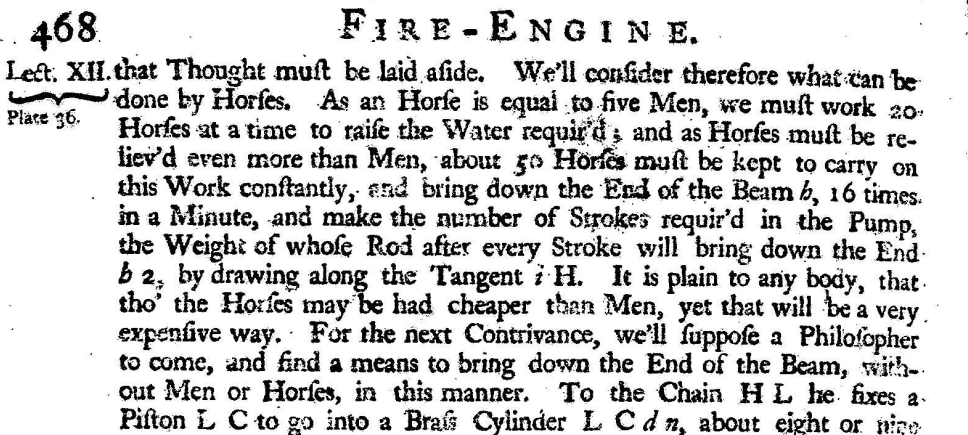
\includegraphics[width=1.05\textwidth]{desagulier2}
%		}
\end{figure}
\end{frame}

\begin{frame}
\frametitle{Real wage to energy ratios\\\textit{Source:} Robert Allen (2009)}
\begin{figure}[p!]
\center
%\caption{Real wage to energy ratios\\\textit{Source:} Robert Allen (2009)}
\label{fig:wage-energy}
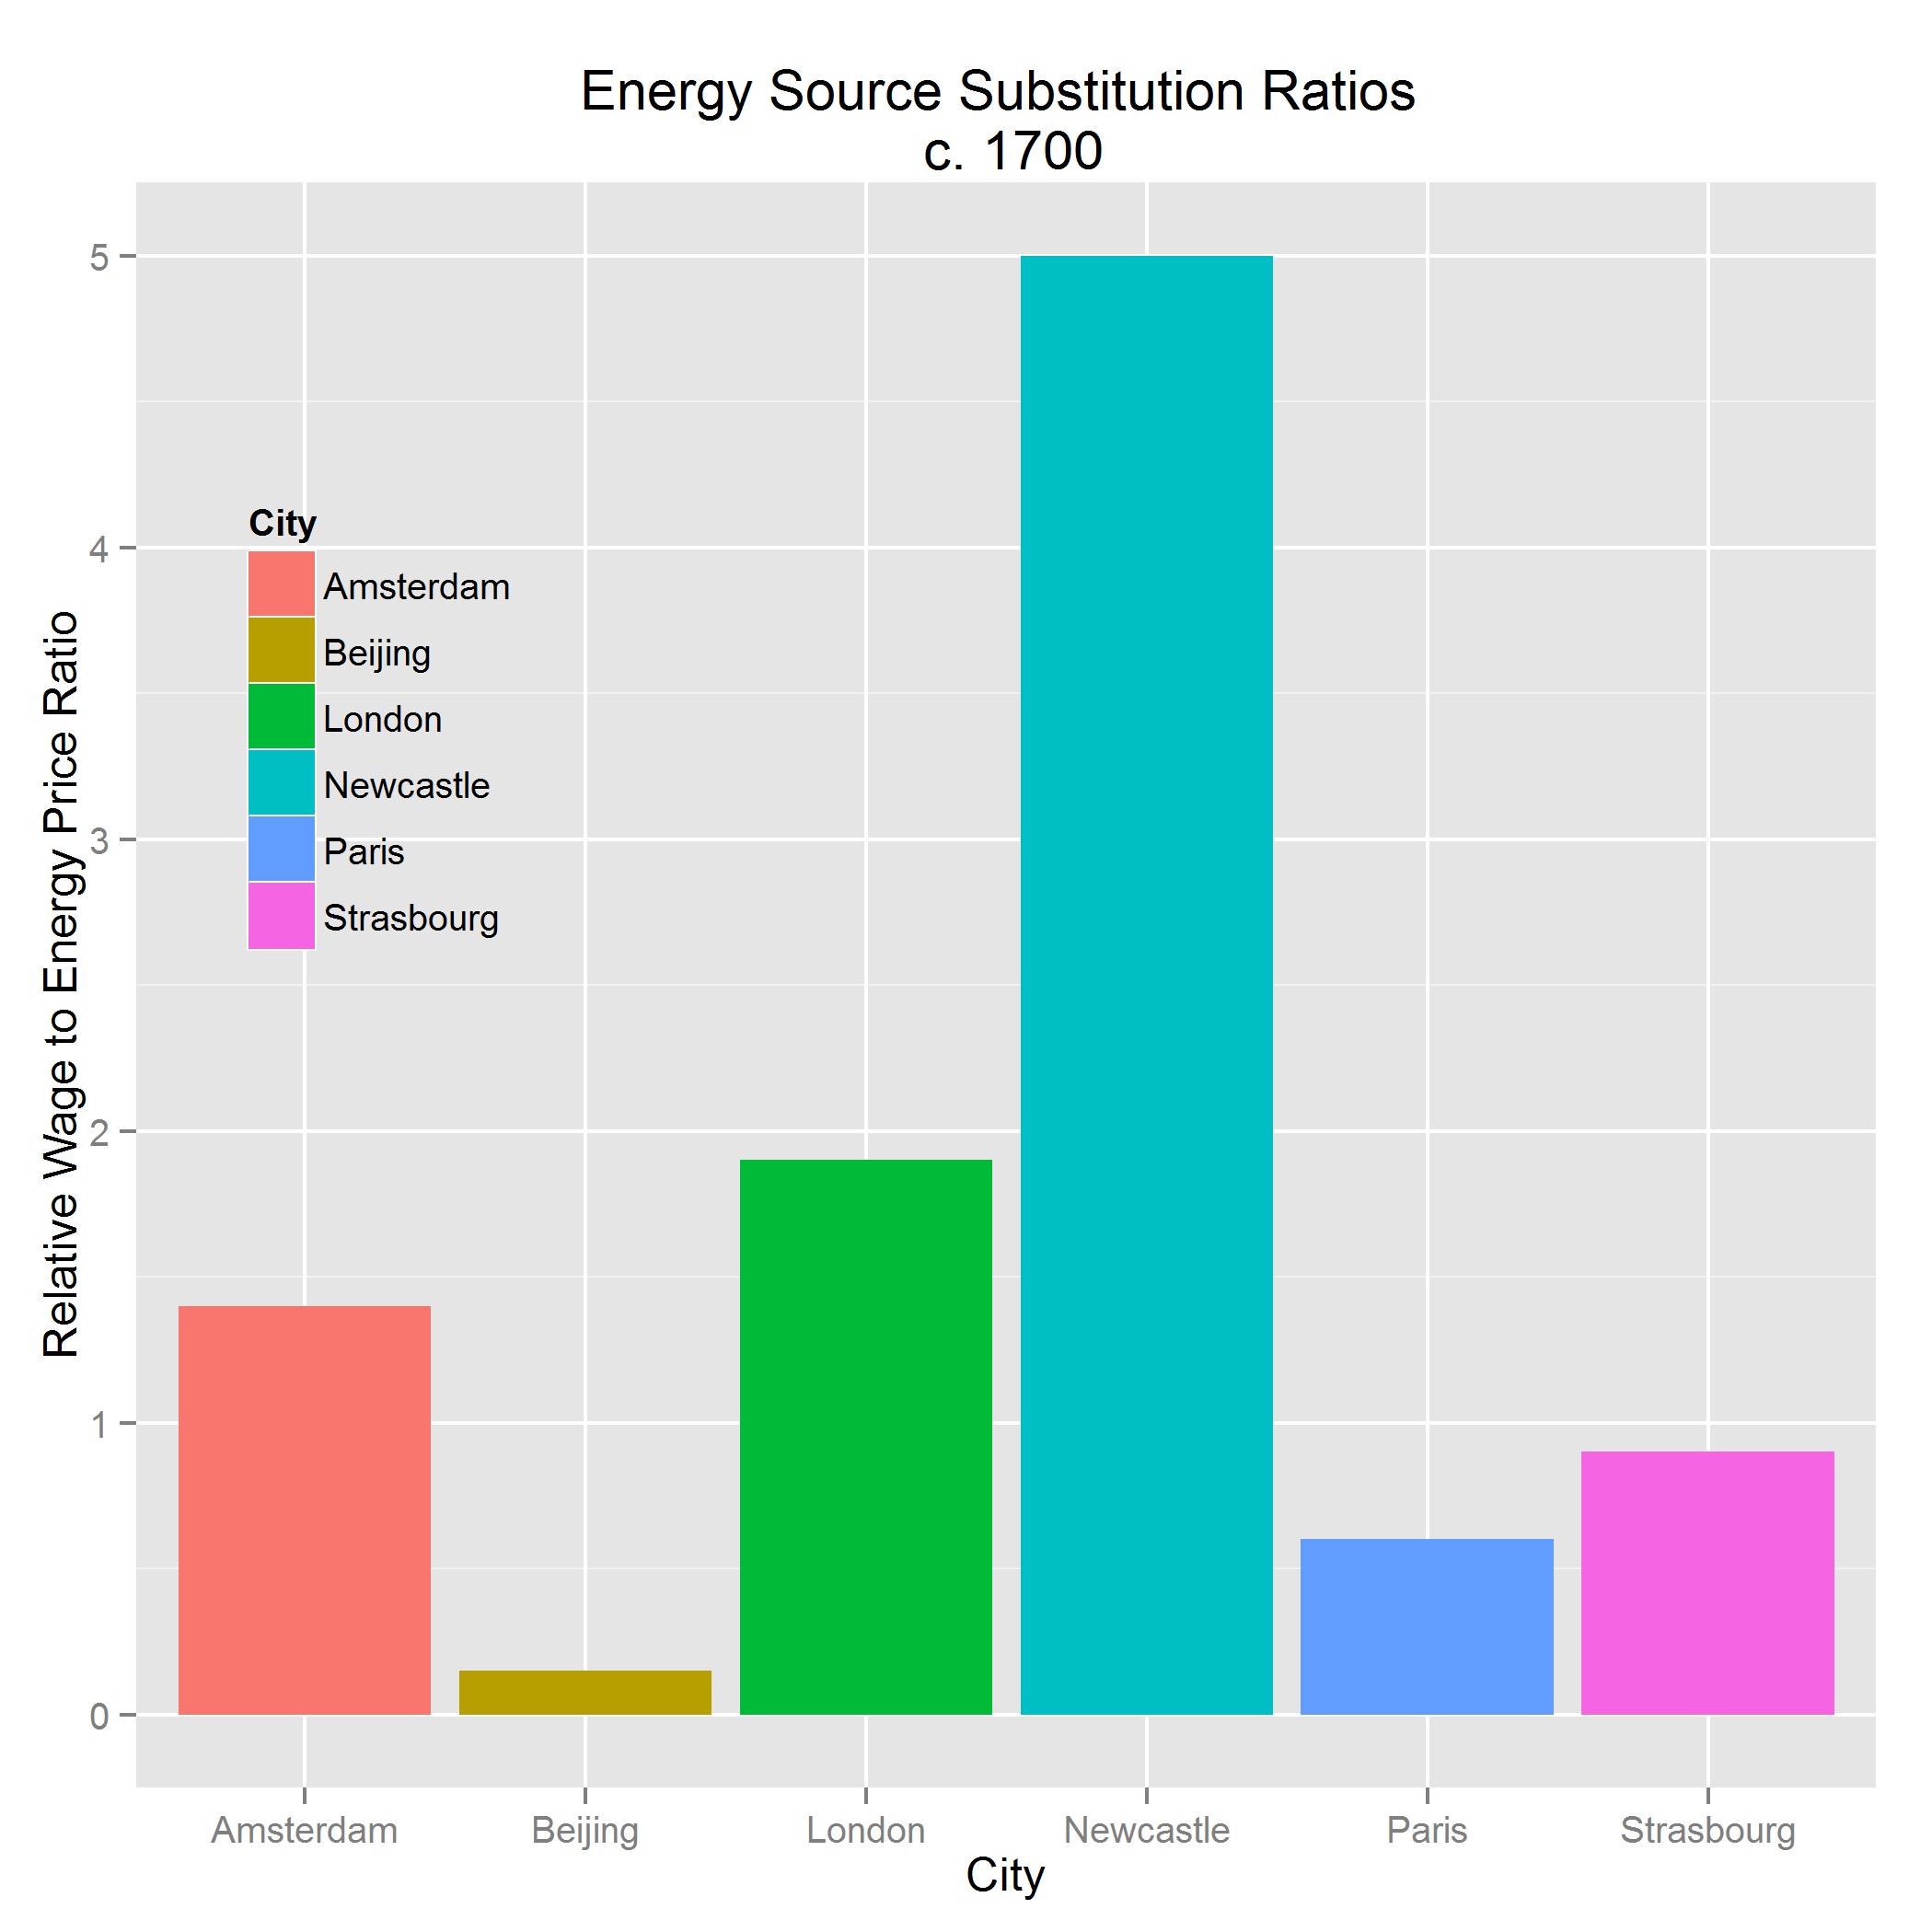
\includegraphics[height=0.8\textheight]{wage-energy.png}
\end{figure}
\end{frame}

\begin{frame}
\frametitle{Microeconomic theory}
\scriptsize{
		\begin{equation}
		\label{eq:mrp}
		\frac{\text{Marginal Revenue Product}_{\text{ organic energy joule}}}{\text{Price}_{\text{ organic energy joule}}} = \frac{\text{Marginal Revenue Product}_{\text{ fossil energy joule}}}{\text{Price}_{\text{ fossil energy joule}}}
		\end{equation}
}
\end{frame}

\begin{frame}
\frametitle{English Industrial Revolution, 1590 - 1876}

	\begin{itemize}
	\item Modern economic growth
	\item Unconstrained quantity of fossil carbon energy -- an \textit{energy} revolution led by a demand revolution
	\item Little statistical space for institutional or cultural events -- except to explain structural breaks
	\item Macro and micro explain a great deal
	\item Framework applicable across time series, space, and time
	\end{itemize}
\end{frame}

\begin{frame}
\frametitle{Thank you}
\end{frame}

\section{Supplement}

\begin{frame}
\frametitle{English wood enegy supply constraint}
\begin{figure}[p!]
\center
%\caption{English wood enegy supply constraint}
\label{fig:wood}
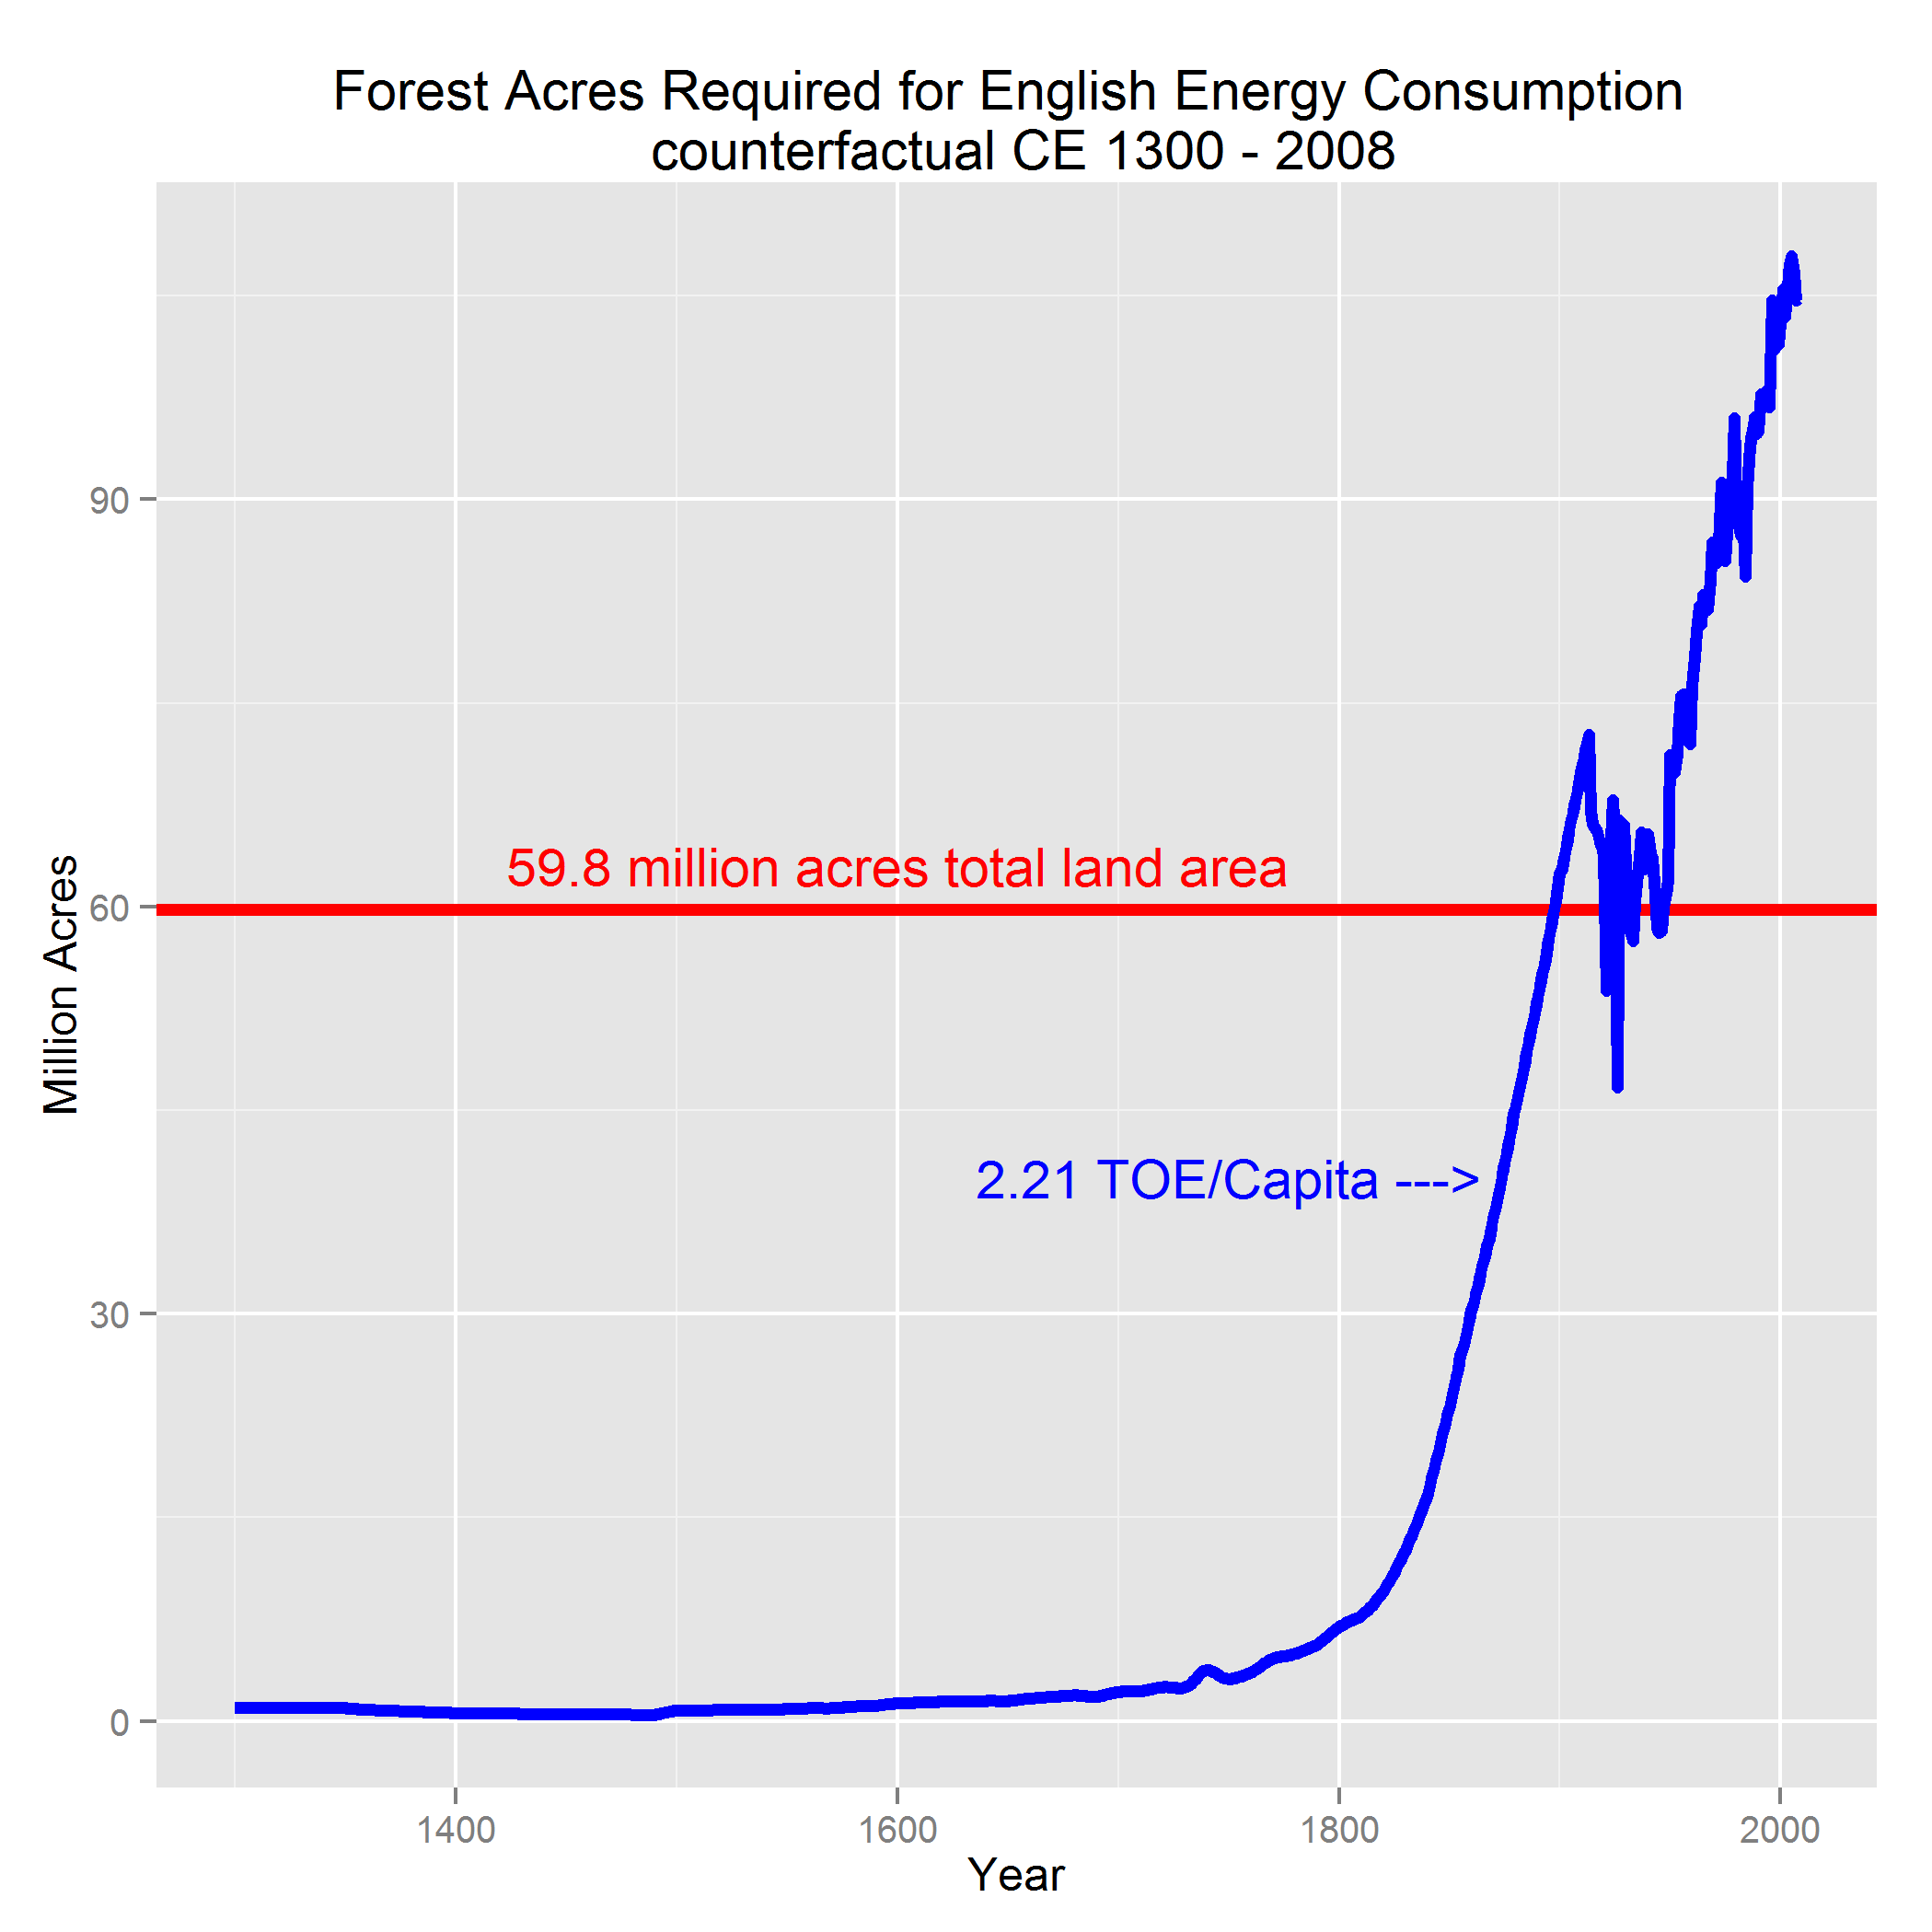
\includegraphics[height=0.8\textheight]{wood}
\end{figure}
\end{frame}

\begin{frame}
\begin{figure}[p!]
\center
\caption{Standardized English energy intensity of GDP}
\label{fig:energyIntensity}
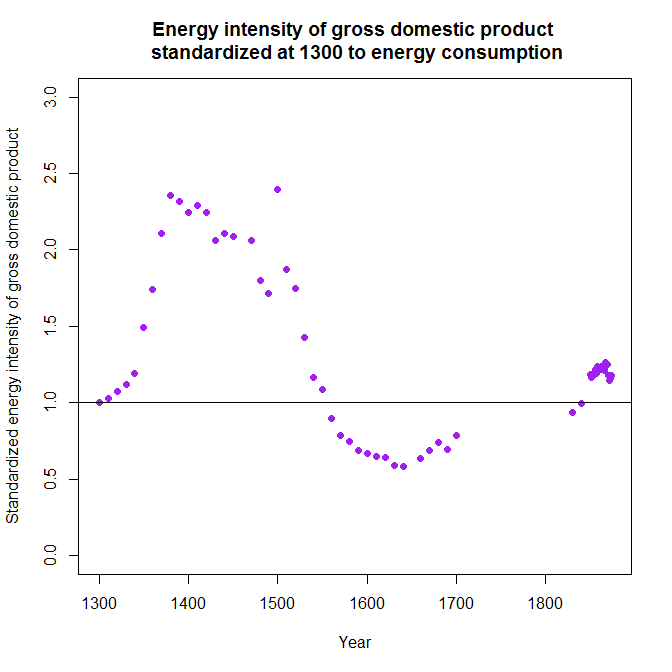
\includegraphics[height=0.8\textheight]{energyIntensity}
\end{figure}
\end{frame}

\begin{frame}
\begin{figure}[p!]
\center
\caption{Log of GDP, with structural breaks}
\label{fig:gbpgdplog.png}
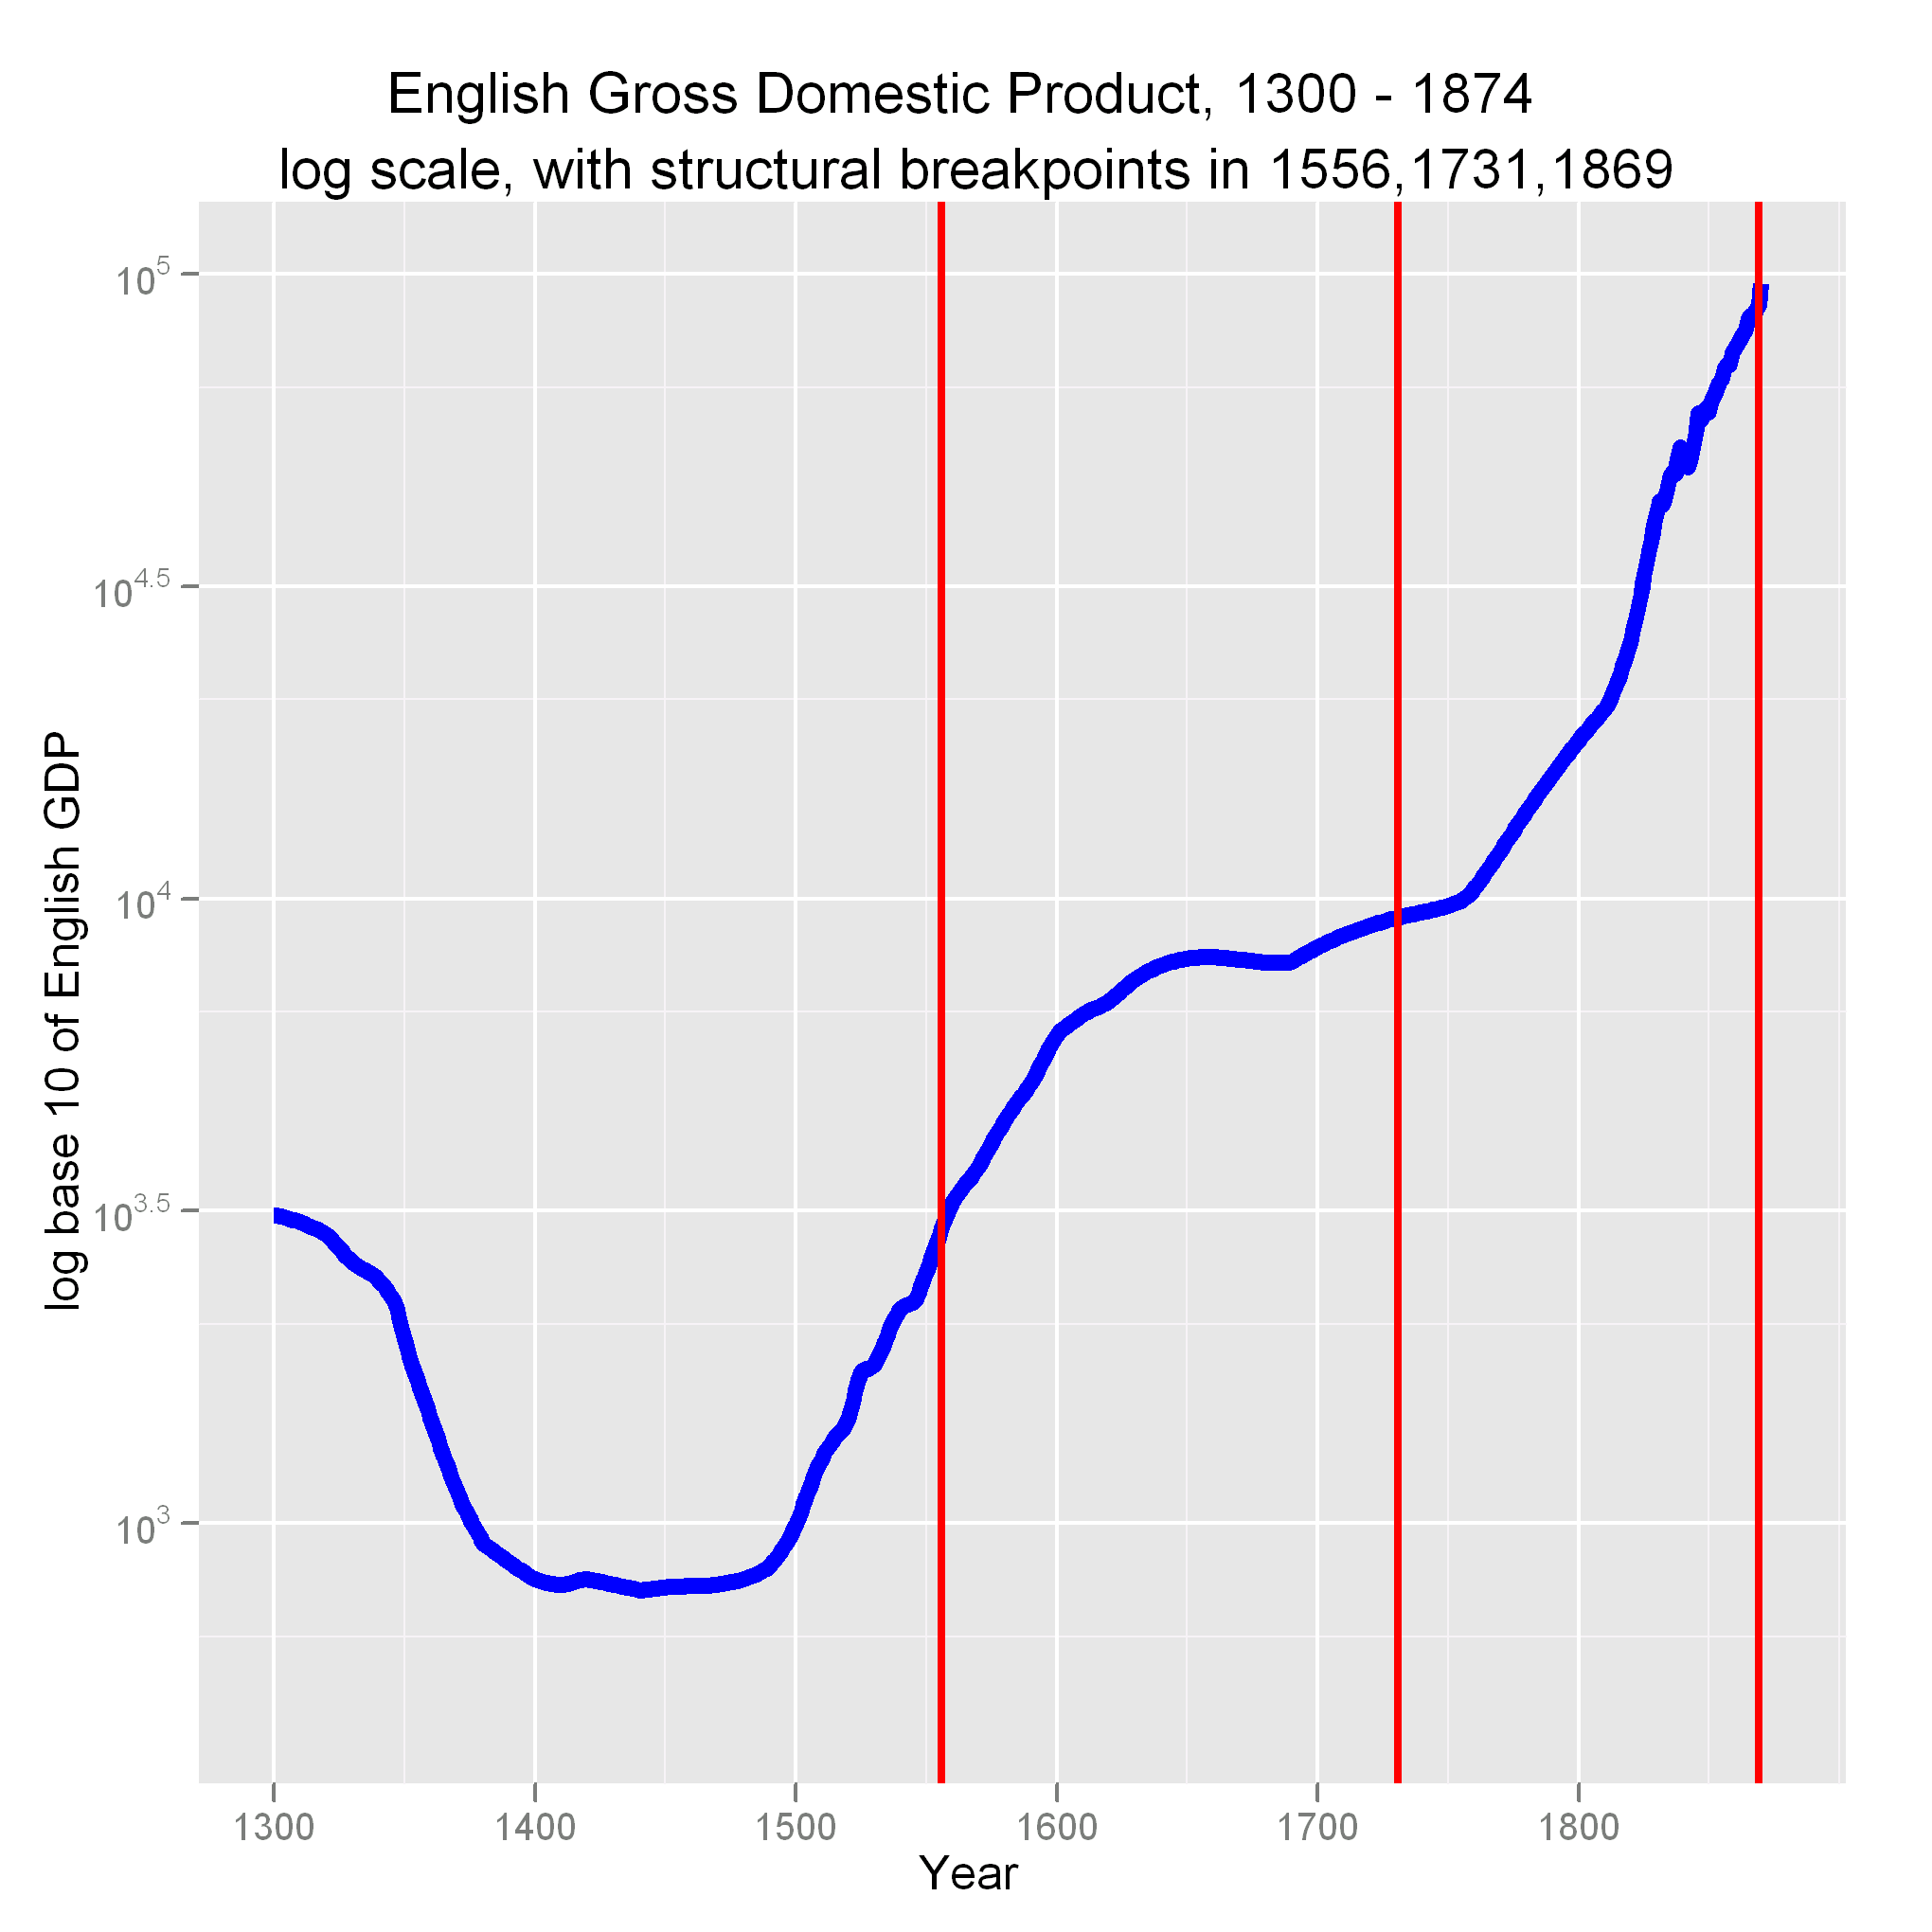
\includegraphics[height=0.8\textheight]{gbpgdplog.png}
\end{figure}
\end{frame}

\begin{frame}
\begin{figure}[p!]
\center
\caption{Log of population, with structural breaks}
\label{fig:popLog}
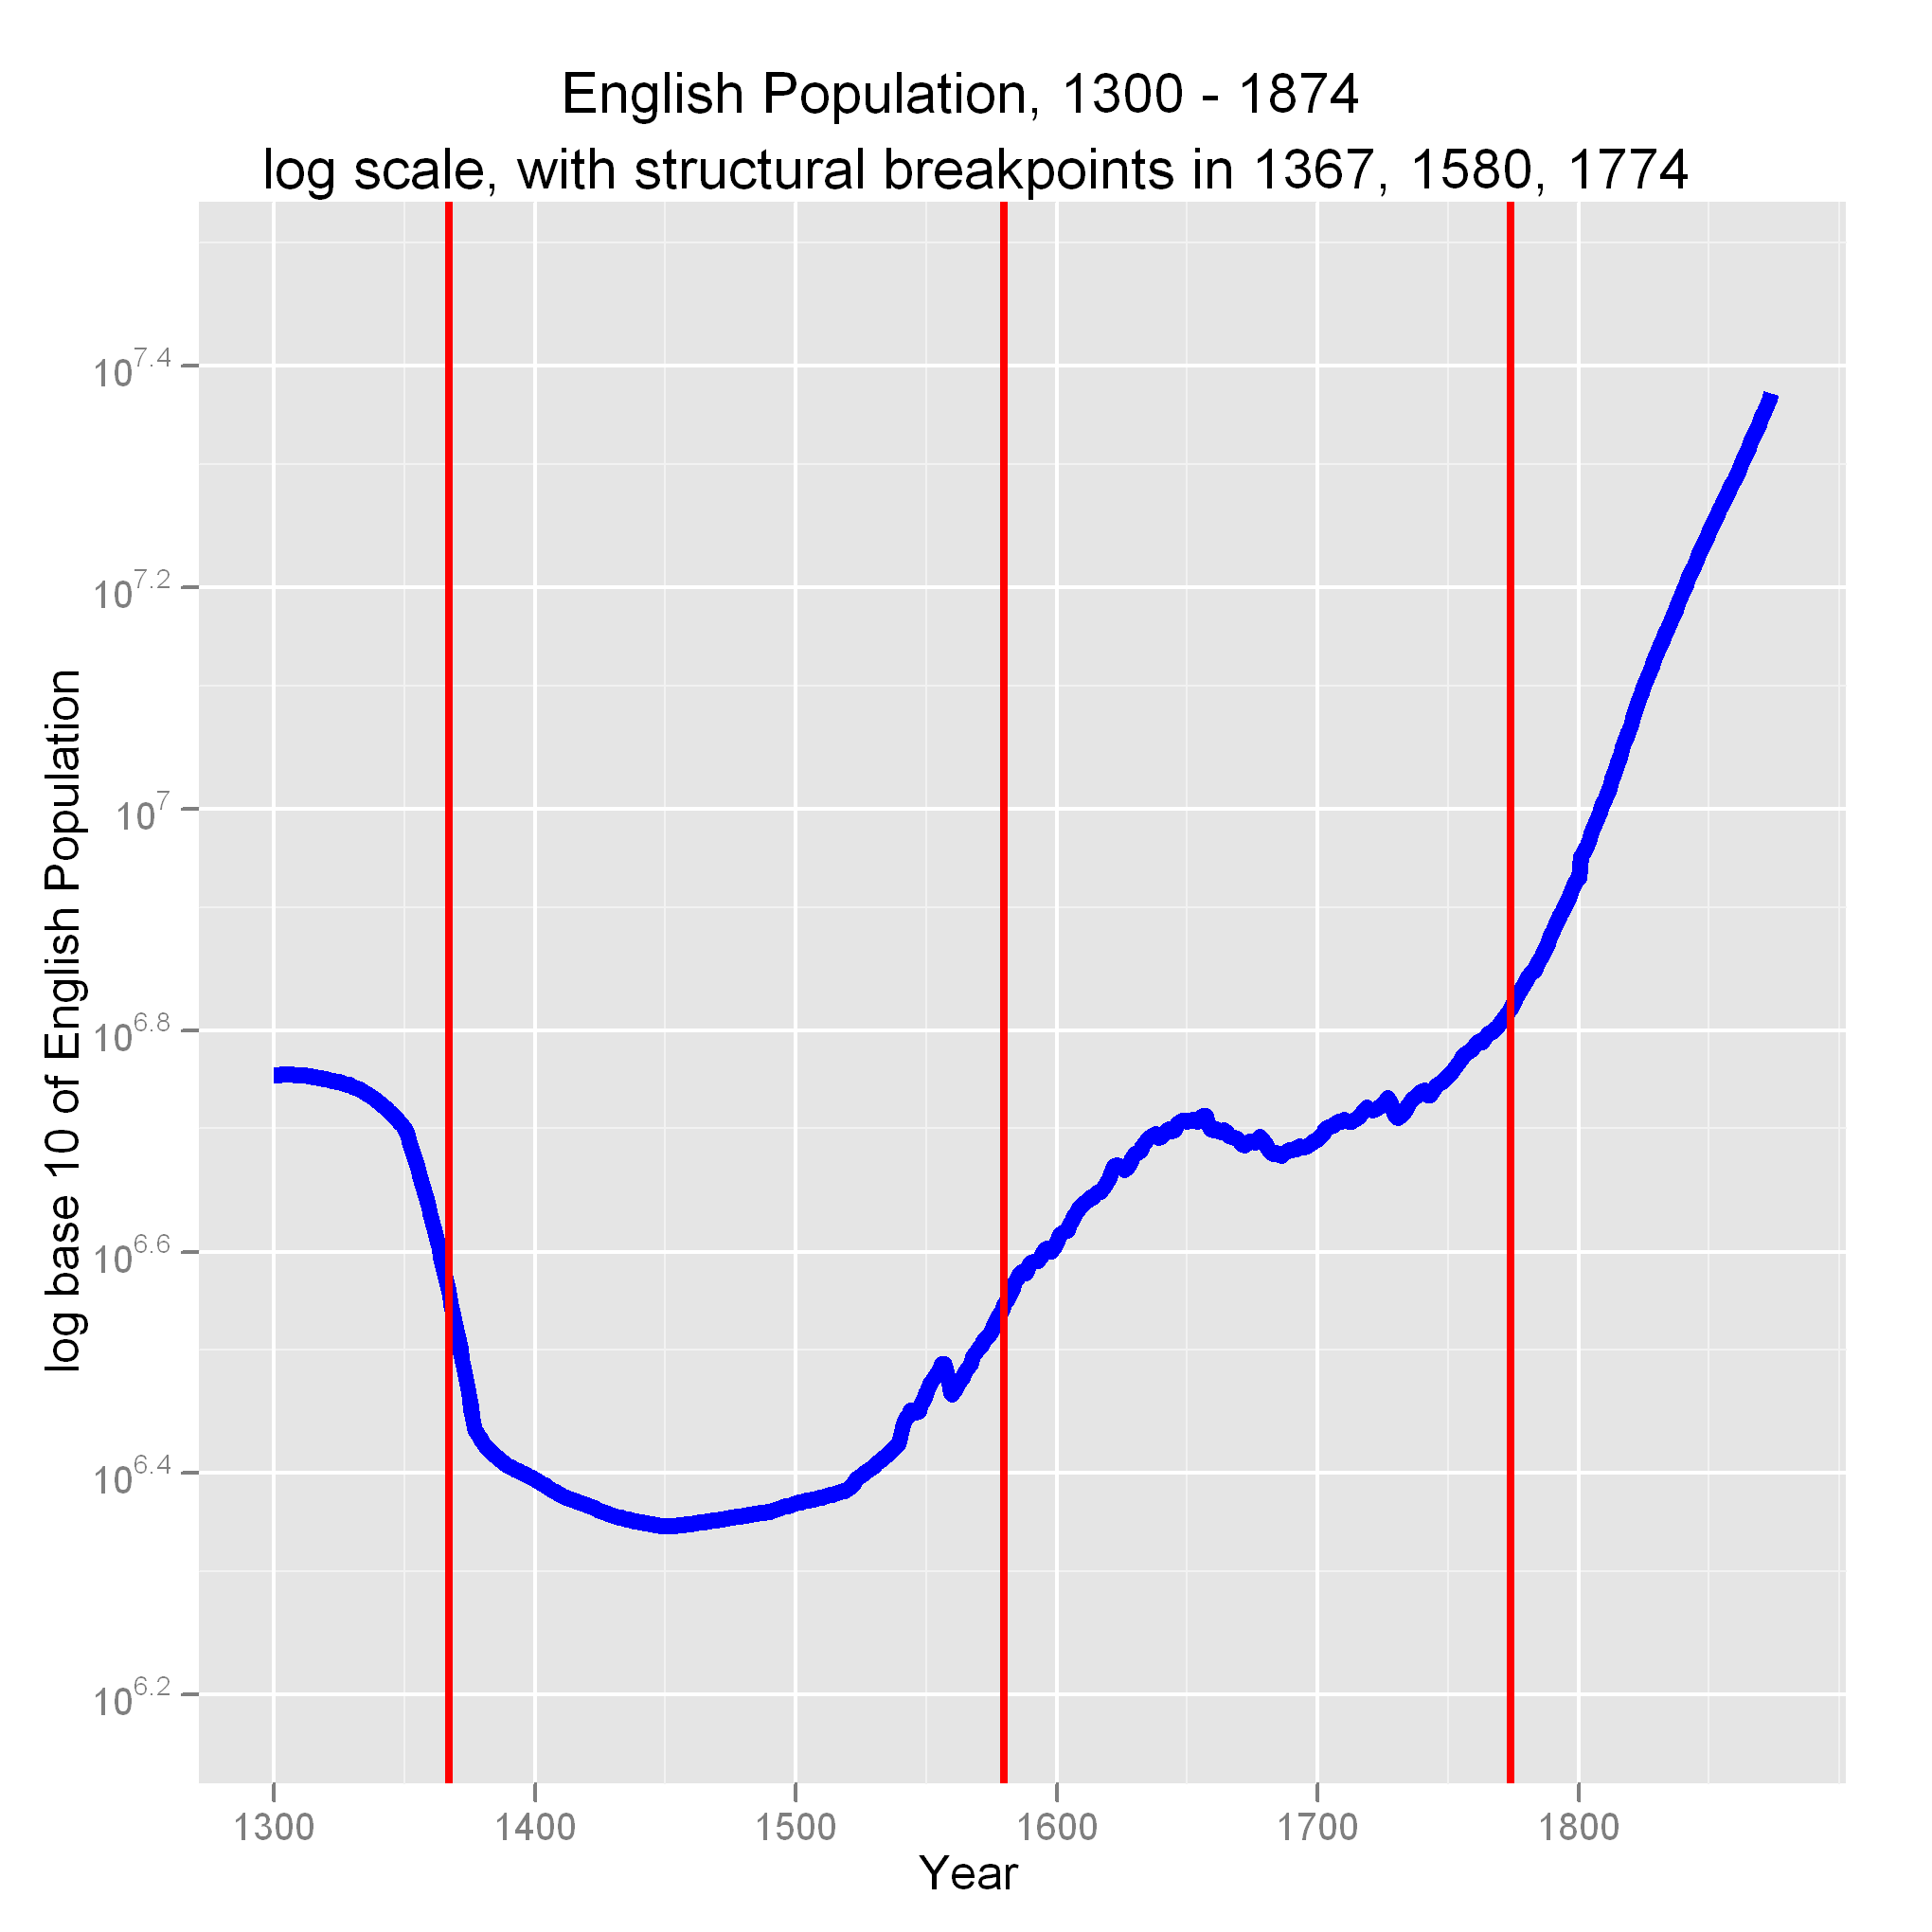
\includegraphics[height=0.8\textheight]{popLog}
\end{figure}
\end{frame}

\begin{frame}
\frametitle{Data Sources}
\footnotesize{
\begin{table}[p!]
%\caption{Data Sources}
\label{tbl:dataSources}
\begin{tabular}{lrll}
Data series&Year range&Geography&Source\\
\hline
Energy consumption&1300 -- 1873&England/Wales&Roger Fouquet (2008)\\
\hline
Gross domestic product&1300 -- 1700&England&Graeme Snooks (1994)\\
&1741 -- 1873&England/Wales&Lawrence Officer (2009)\\
\hline
Population&1300 -- 1540&England&Graeme Snooks (1994)\\
&1541 -- 1800&England&B. R. Mitchell (1988)\\
&1801 -- 1873&England/Wales&B. R. Mitchell (1988)\\
\end{tabular}
\end{table}
}
\end{frame}

\begin{comment}
\begin{table}[p!]
\caption{t-test of energy and gdp}
\label{tbl:t-testEnergyGdp}
\begin{tabular}{rl}
\end{tabular}
\end{table}
\end{comment}

\begin{frame}
\tiny{
\begin{table}[p!]
\caption{growth rates by century}
\label{tbl:growthByCentury}
\begin{tabular}{lrrrrrrrr}
Year	&	1300	&	1400	&	1500	&	1600	&	1700	&	1801	&	1873&Total	\\
\hline
GDP Million\\ 2005 GBP	&	3114.7541	&	815.1288	&	994.4571	&	6031.953	&	8361.5911	&	18110	&	102811&	\\
Century-over-century\\rate of growth&&-0.738&0.220&5.066&0.386&1.166&4.677&32.008\\
Compounded annual \\rate of growth&&-0.013&0.002&0.018&0.003&0.008&0.024&0.006\\
\hline
Energy consumption&1.7	&	1	&	1.3	&	2.2	&	3.6	&	11.6	&	66.1&	\\
Century-over-century\\rate of growth&&-0.412&0.300&0.692&0.636&2.222&4.698&37.882\\
Compounded annual \\rate of growth&&-0.005&0.0026&0.005&0.005&0.012&0.024&0.006\\
\hline
Per-capita GDP\\2005 GBP&542&  329&  421& 1,484& 1,663& 1,999& 4,392\\
Century-over-century\\rate of growth&&-0.393& 0.282&2.521&0.121&0.202&1.198& 7.108\\
Compounded annual \\rate of growth&&-0.005&0.002&0.013&0.001&0.002& 0.011&0.004\\
\end{tabular}
\end{table}
}
\end{frame}

\begin{frame}
\begin{table}[p!]
\caption{Energy and GDP fit tests}
\label{tbl:fitTest}
\begin{center}
\begin{tabular}{lrr}
\hline\hline
Test&Statistic&p-value\tabularnewline
\multicolumn{1}{c}{}\tabularnewline
\hline
Pearson's correlation&$0.998$&\tabularnewline
\hline
Paired t-test&$5.592$&4.991e-07\tabularnewline
\hline
Chi-square&2864&0.0004998\tabularnewline
\end{tabular}
\end{center}
\end{table}
\end{frame}



\end{document}